\documentclass{article}
\usepackage[UTF8]{CTEX}
\usepackage{hyperref}
\usepackage{geometry}
\usepackage{graphicx}
\usepackage{subfig}

\geometry{a4paper, left=3cm, right=3cm, top=3cm, bottom=3cm}

\title{Chat Free APP开发手册}
\author{Koorye}
\date{2024.7.1}

\begin{document}

\maketitle
\begin{center}
本应用全部代码开源,可在\href{https://github.com/Koorye/ChatFree}{github.com/Koorye/ChatFree}查看
\end{center}

\section{前言}

Chat Free是一款全平台的AI聊天APP,支持不同大语言模型API的调用,用户可以定义不同的角色,实现多角色聊天。之所以开发本APP,是因为现有的AI聊天APP限制极大且难以定制,而且通常需要收费,不能满足用户的需求,本APP的目标是提供一个全新的聊天体验。

本APP具有以下特点:

\begin{itemize}
    \item 高度定制化的角色。Chat Free支持用户自定义角色,用户可以自己定义角色的名字、性别、年龄、职业等信息。
    \item 灵活调节的API。Chat Free支持用户调节不同的API,用户可以根据自己的需求选择不同的API。
    \item 多角色随时切换的聊天。Chat Free支持用户随时切换不同的角色进行聊天,实现多角色的聊天体验。
    \item 对话历史。Chat Free支持用户保存对话,用户可以随时打开或关闭之前的对话。
    \item 记忆功能。Chat Free支持LLM是否记忆先前的对话,从而作出不同的反应。
    \item 多平台支持。Chat Free支持多平台,用户可以在不同的设备上使用Chat Free。
    \item 免费使用。Chat Free是一款免费APP,用户可以免费使用Chat Free。
\end{itemize}

总之,Chat Free是一款全新的AI聊天APP,希望能够给用户带来全新的聊天体验。

\section{开发环境}

Chat Free APP基于以下环境开发:

\begin{itemize}
    \item 操作系统:Windows 11
    \item 开发工具:HBuilder X 4.15
    \item 编程语言:HTML、CSS、JavaScript
    \item 开发框架:Vue3、Vite 5.2.8、Uniapp
    \item API: 百度ERNIE tiny/speed、讯飞Spark lite
\end{itemize}

\section{APP演示}

\subsection{总体页面}

% 多子图并排:pics/agreement.jpg, pics/chat.jpg, pics/role.jpg, pics/config.jpg
\begin{figure}[h]
    \centering
    \subfloat[用户协议页面]{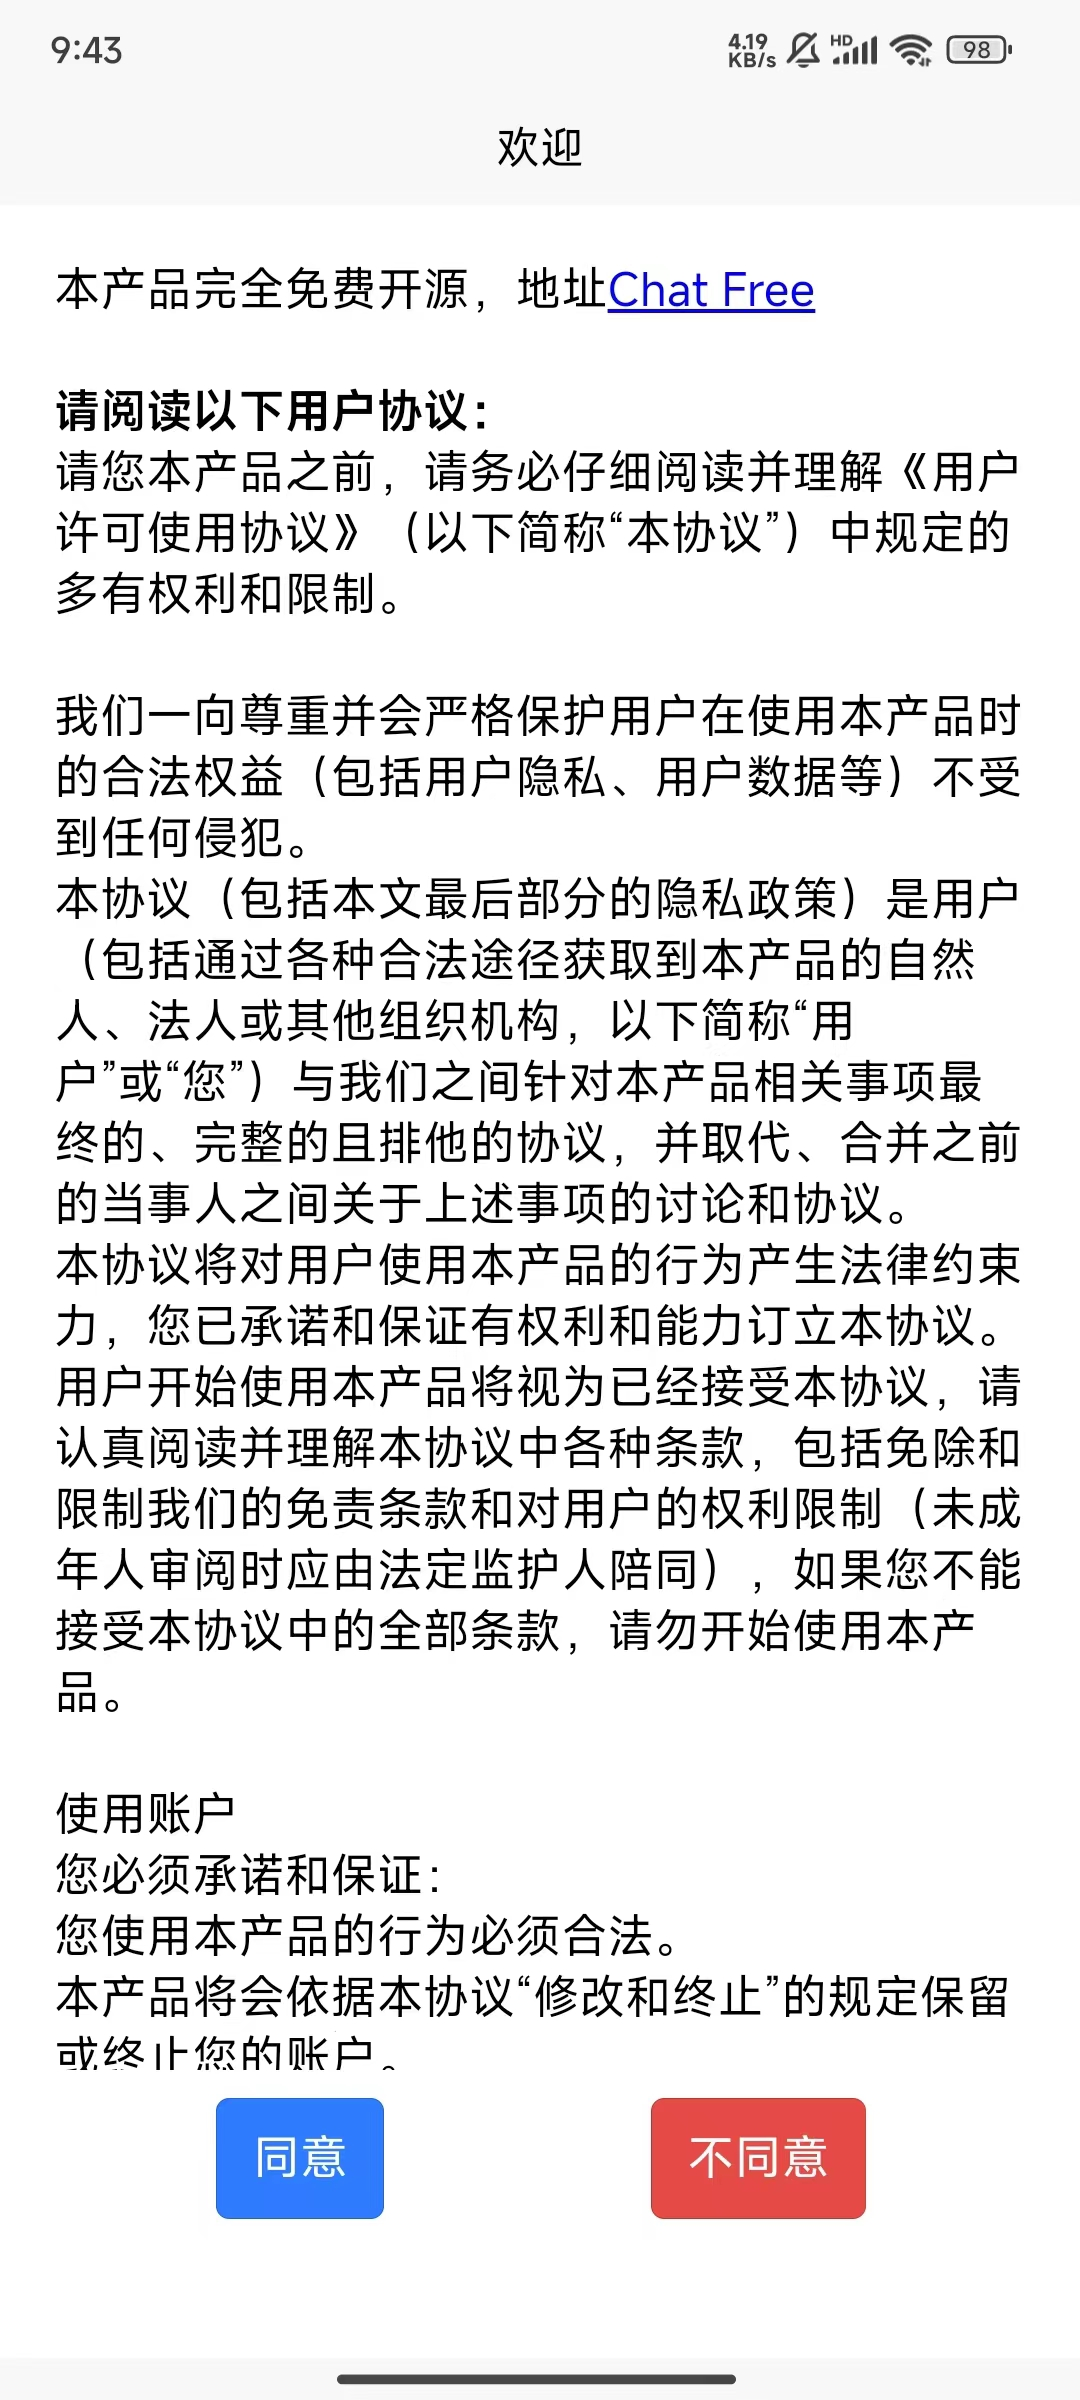
\includegraphics[width=0.3\textwidth]{pics/agreement.jpg}}
    \subfloat[对话设置页面]{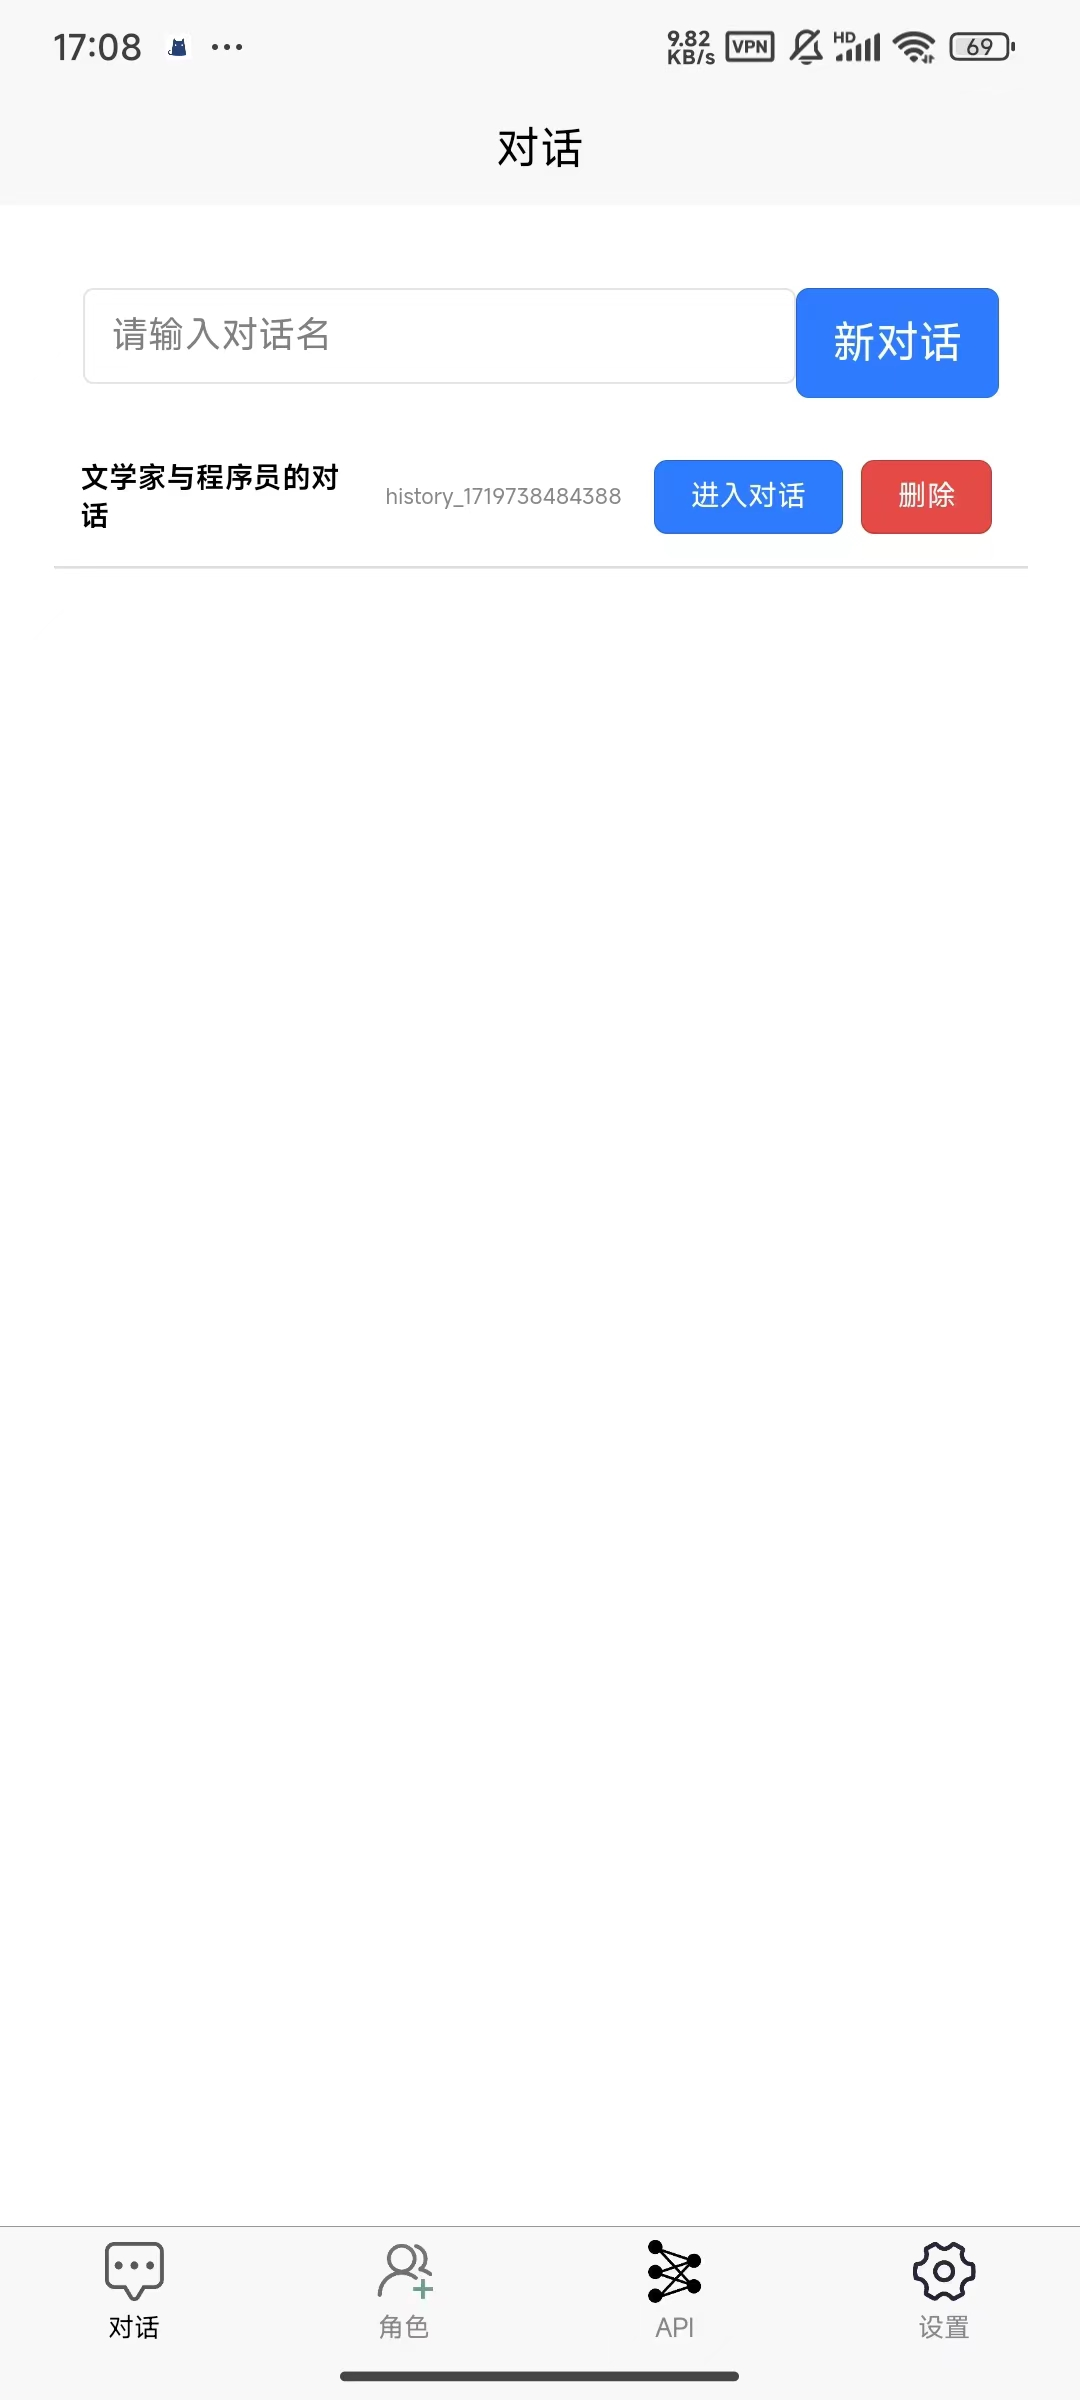
\includegraphics[width=0.3\textwidth]{pics/chat.jpg}}
    \subfloat[角色设置页面]{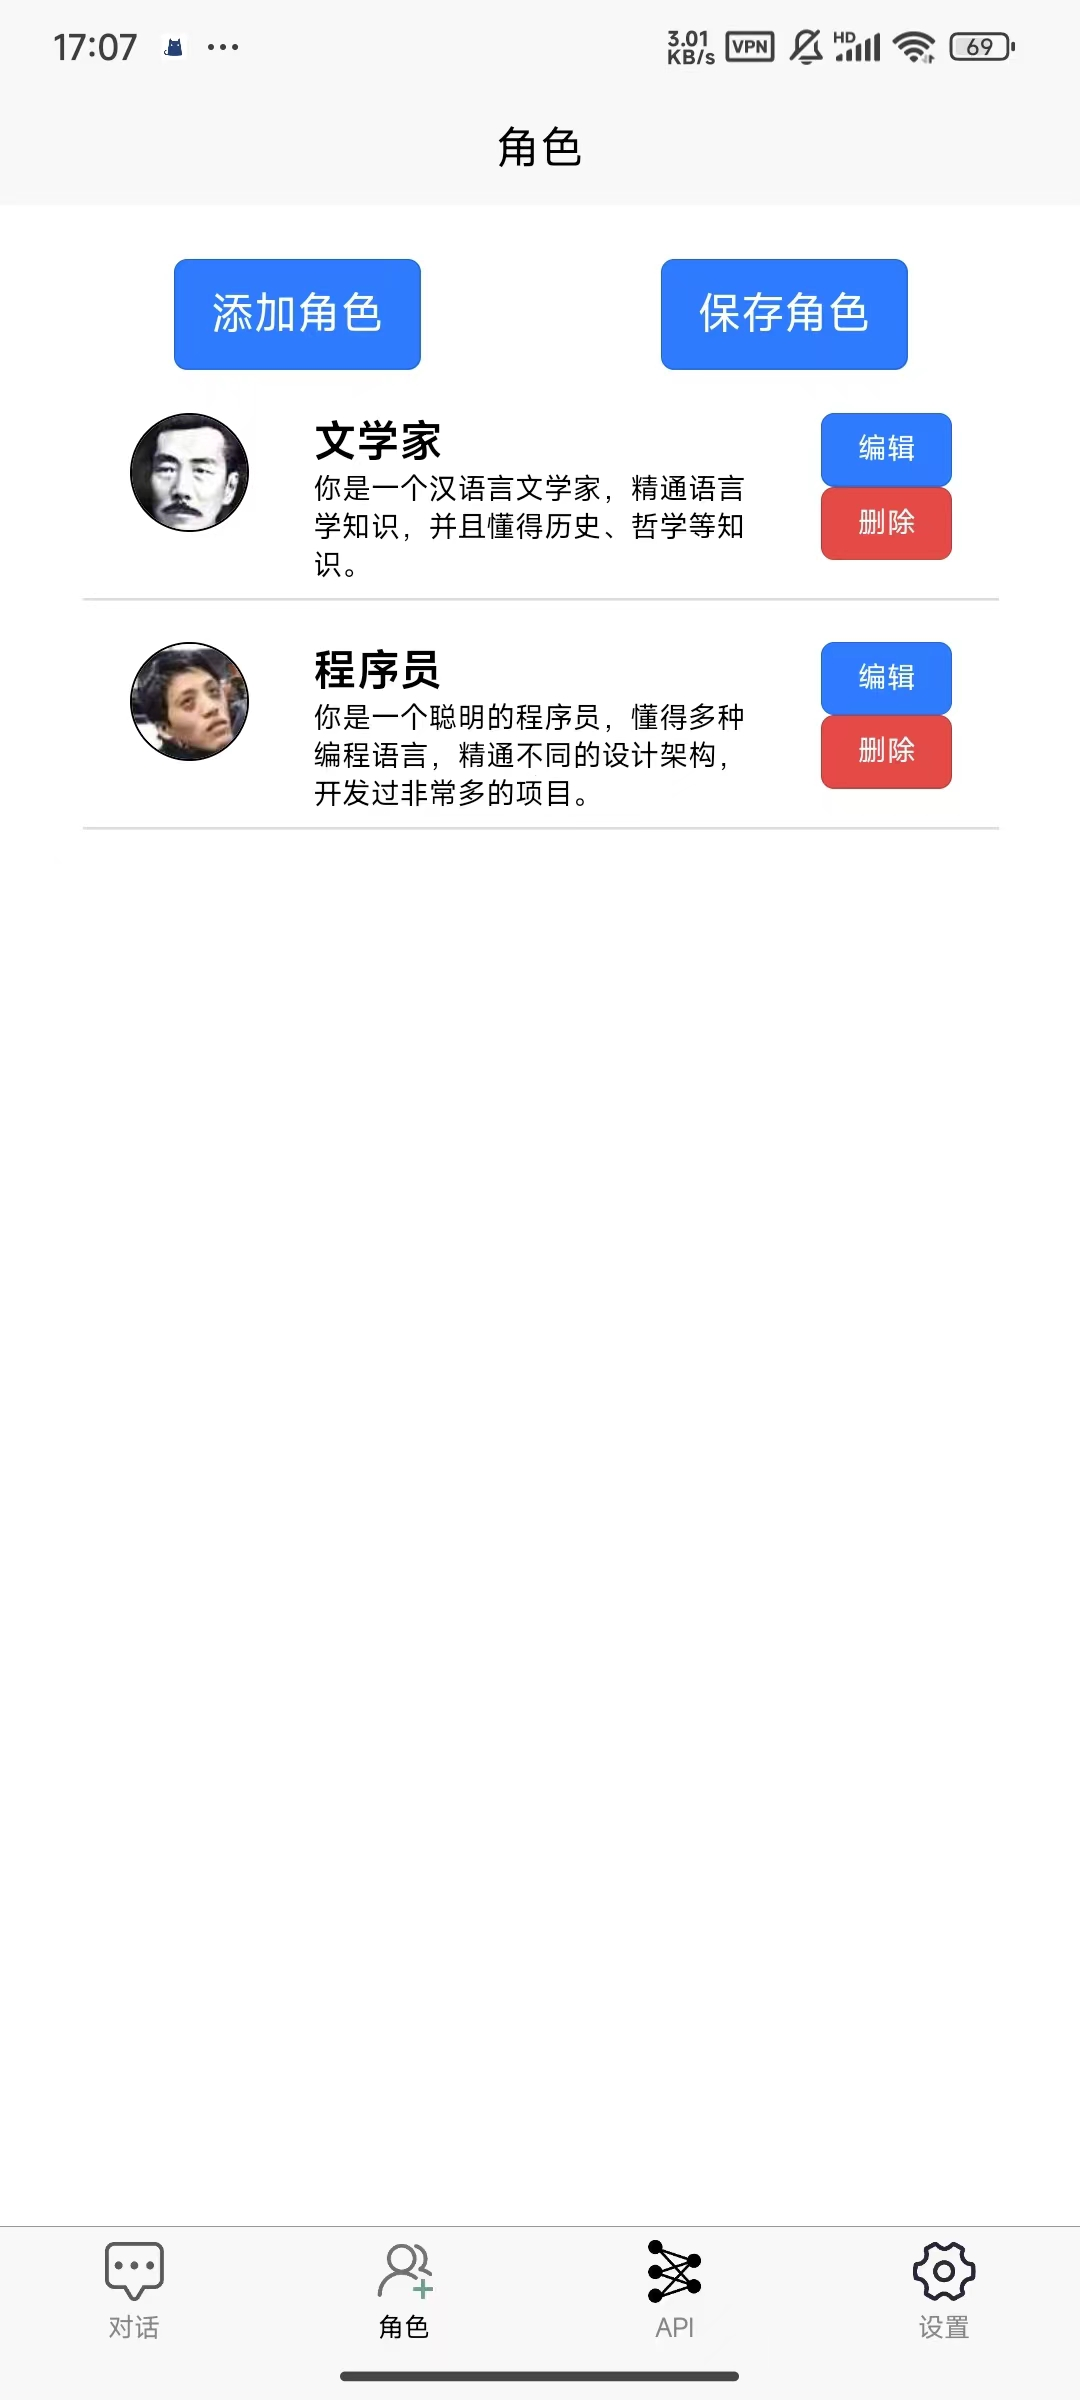
\includegraphics[width=0.3\textwidth]{pics/role.jpg}}
    \caption{Chat Free APP总体页面}
    \label{fig:total}
\end{figure}

\begin{figure}[h]
    \centering
    \subfloat[API设置页面]{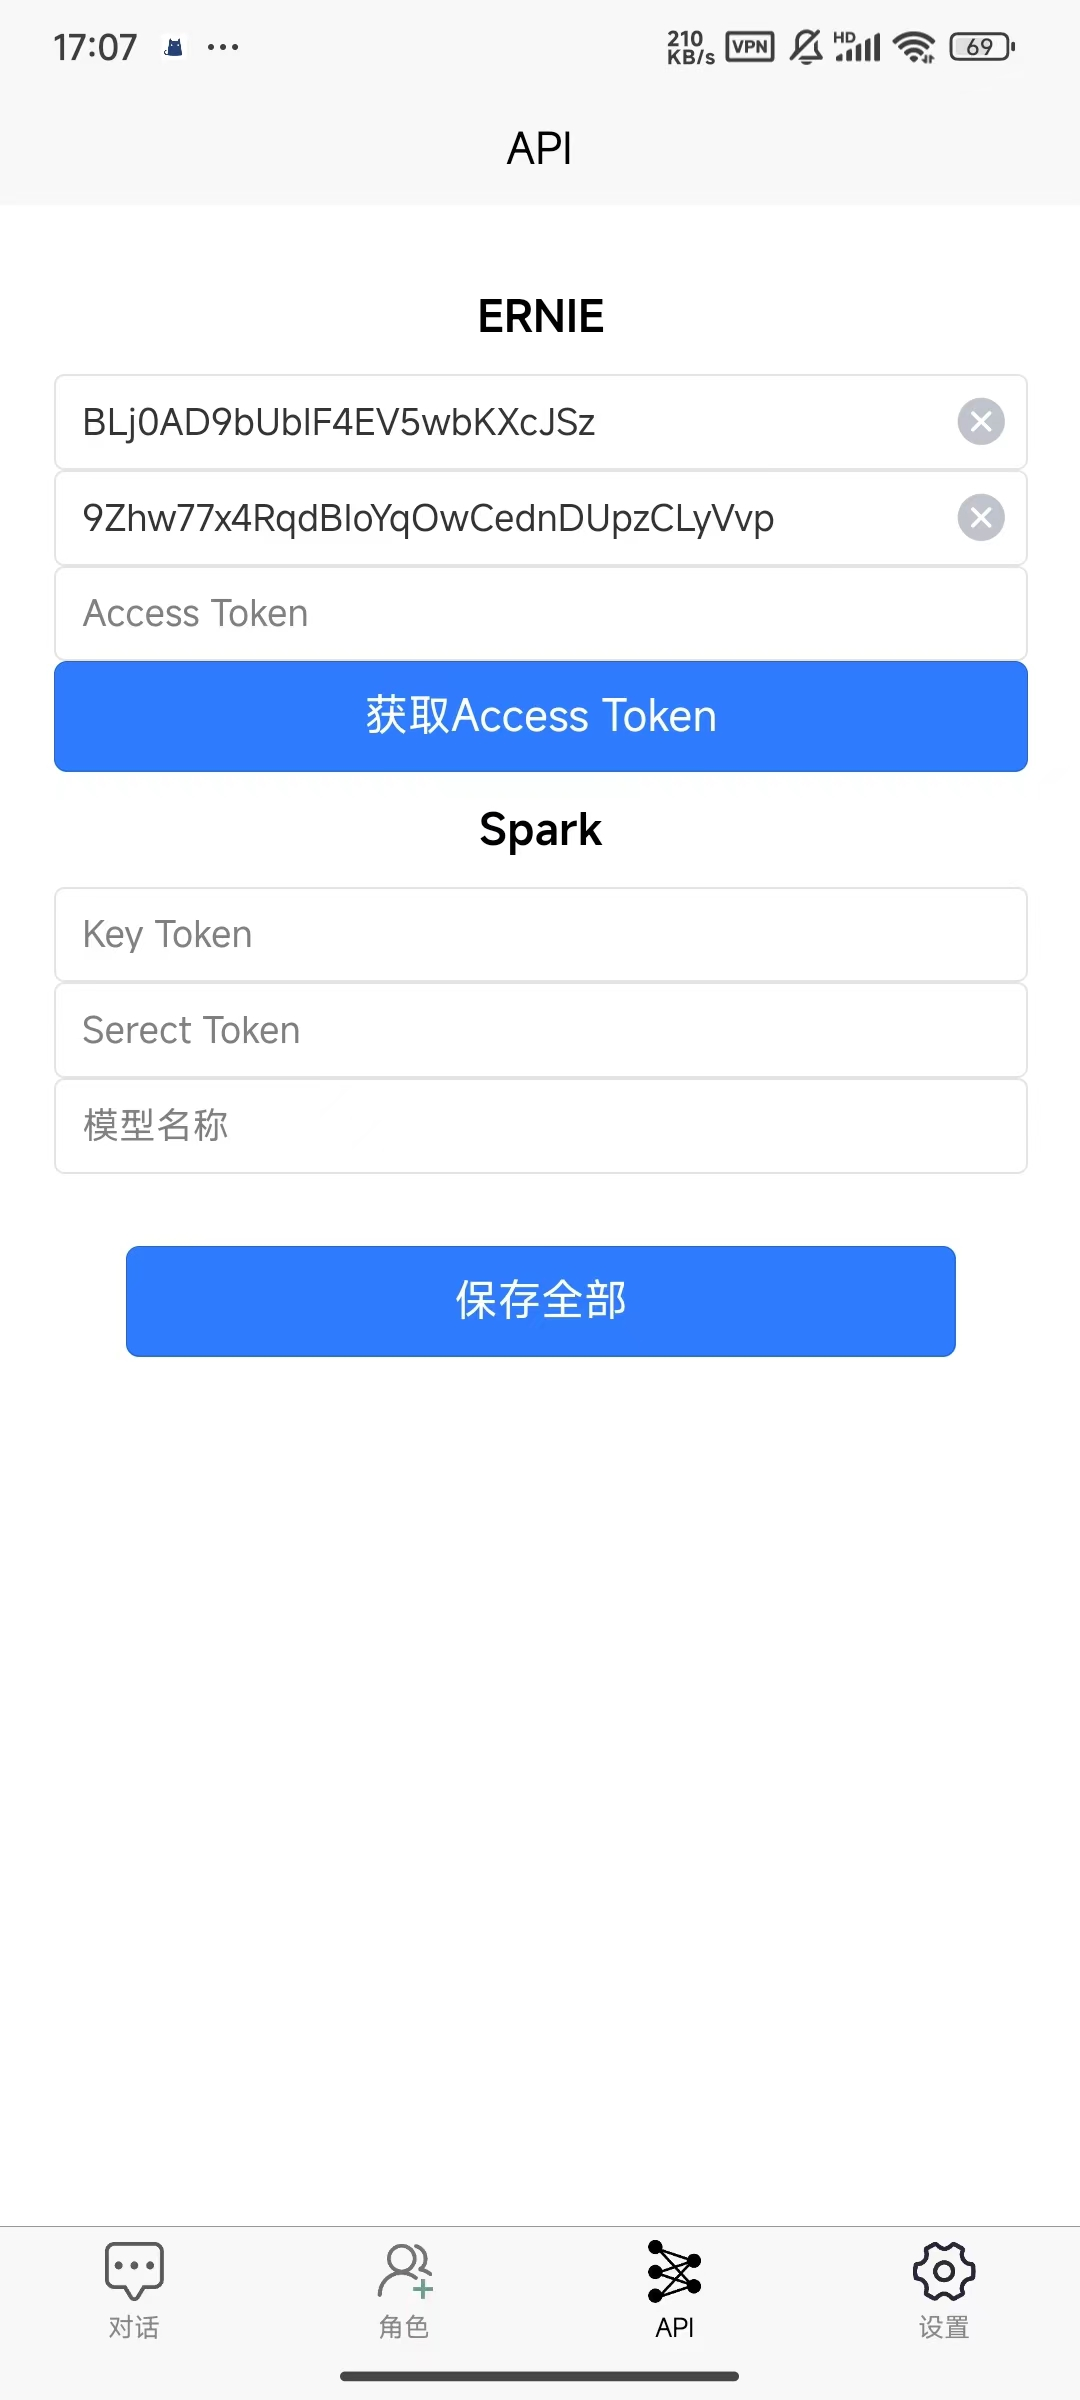
\includegraphics[width=0.3\textwidth]{pics/api.jpg}}
    \subfloat[设置页面]{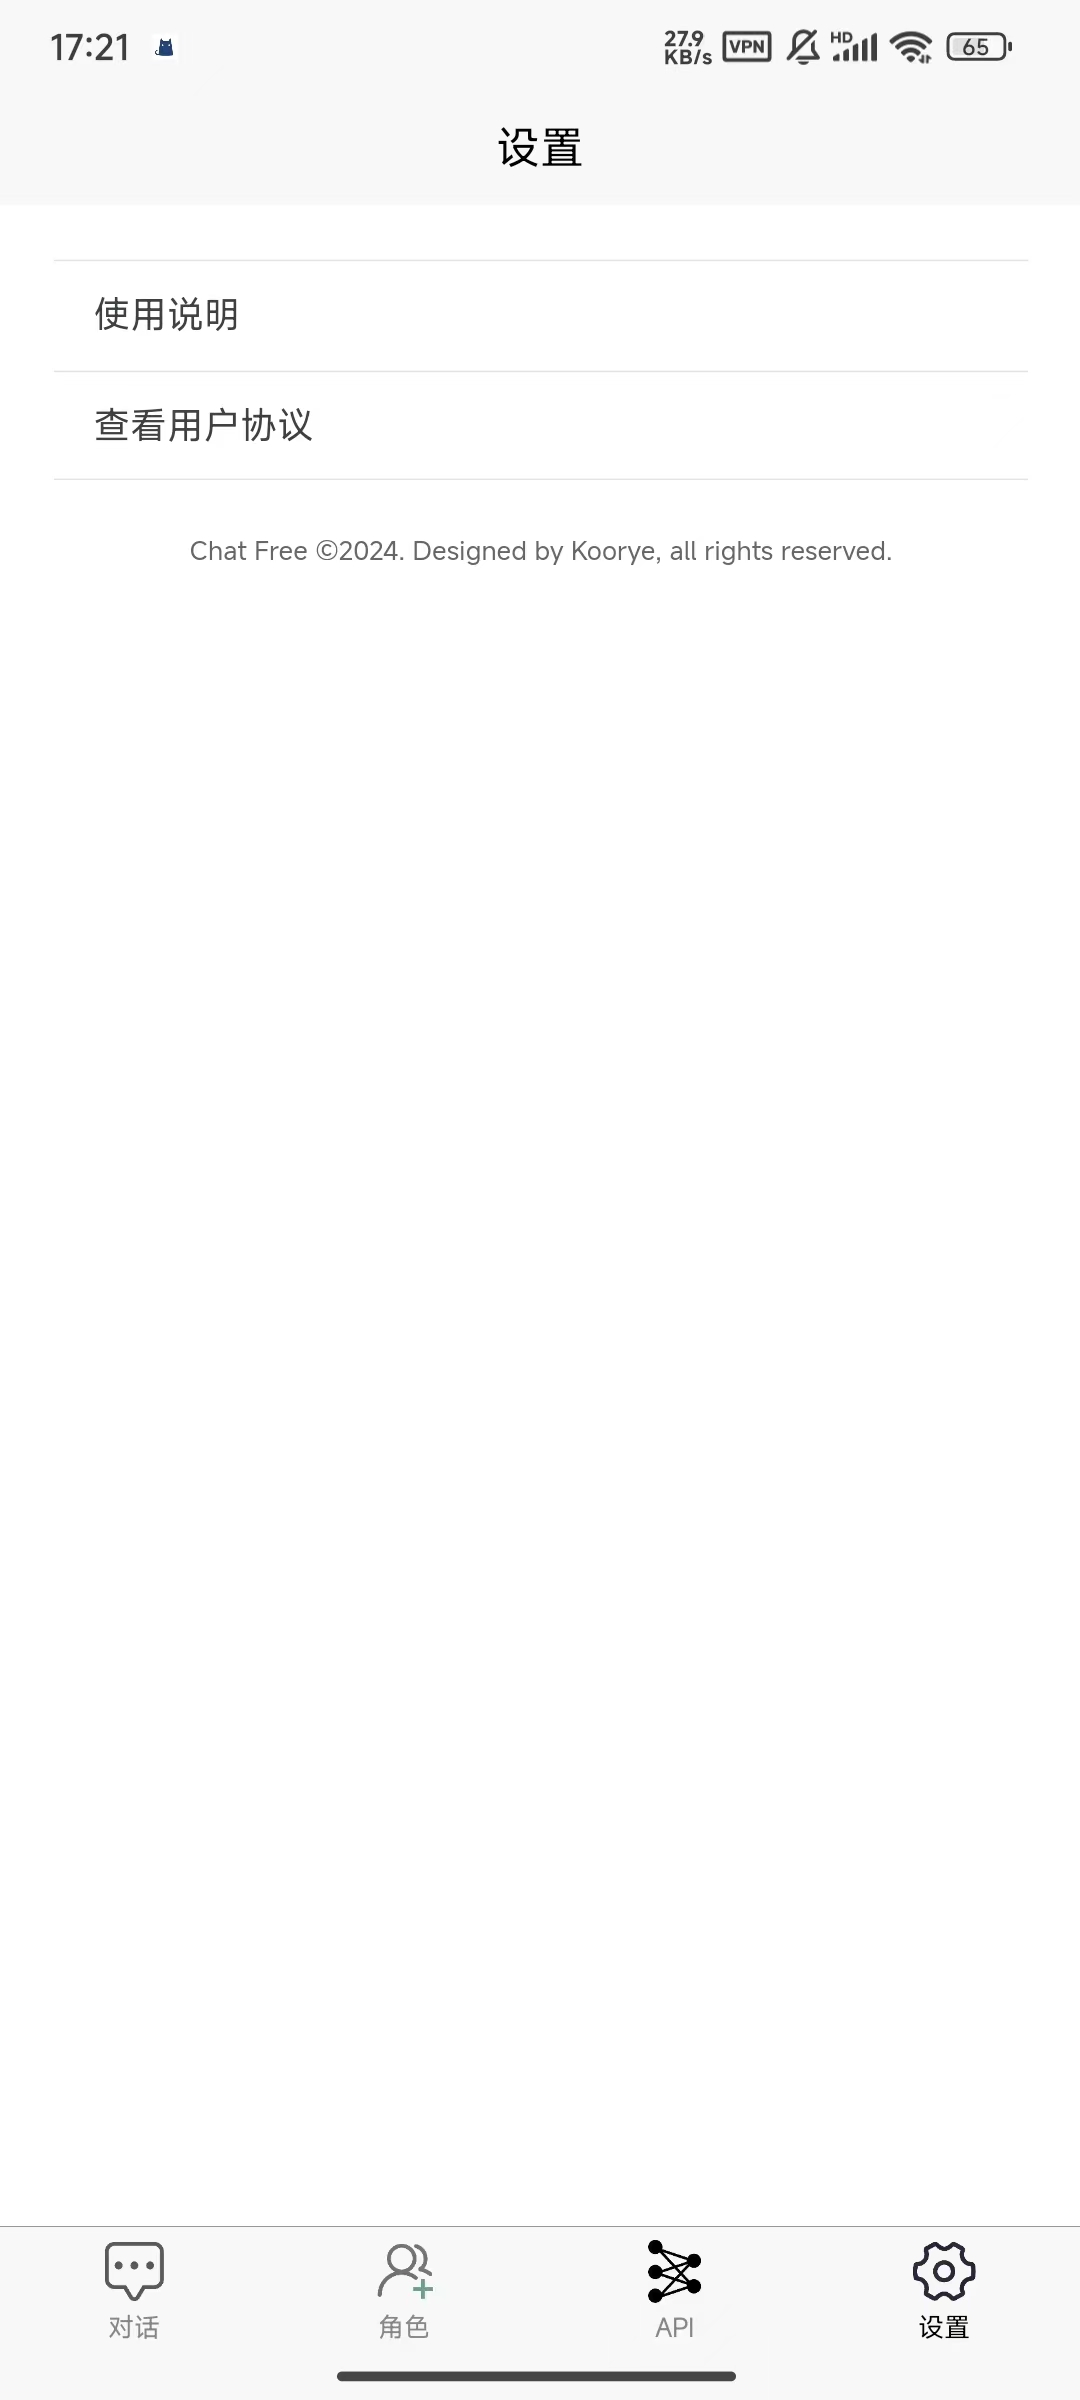
\includegraphics[width=0.3\textwidth]{pics/config.jpg}}
    \subfloat[聊天页面]{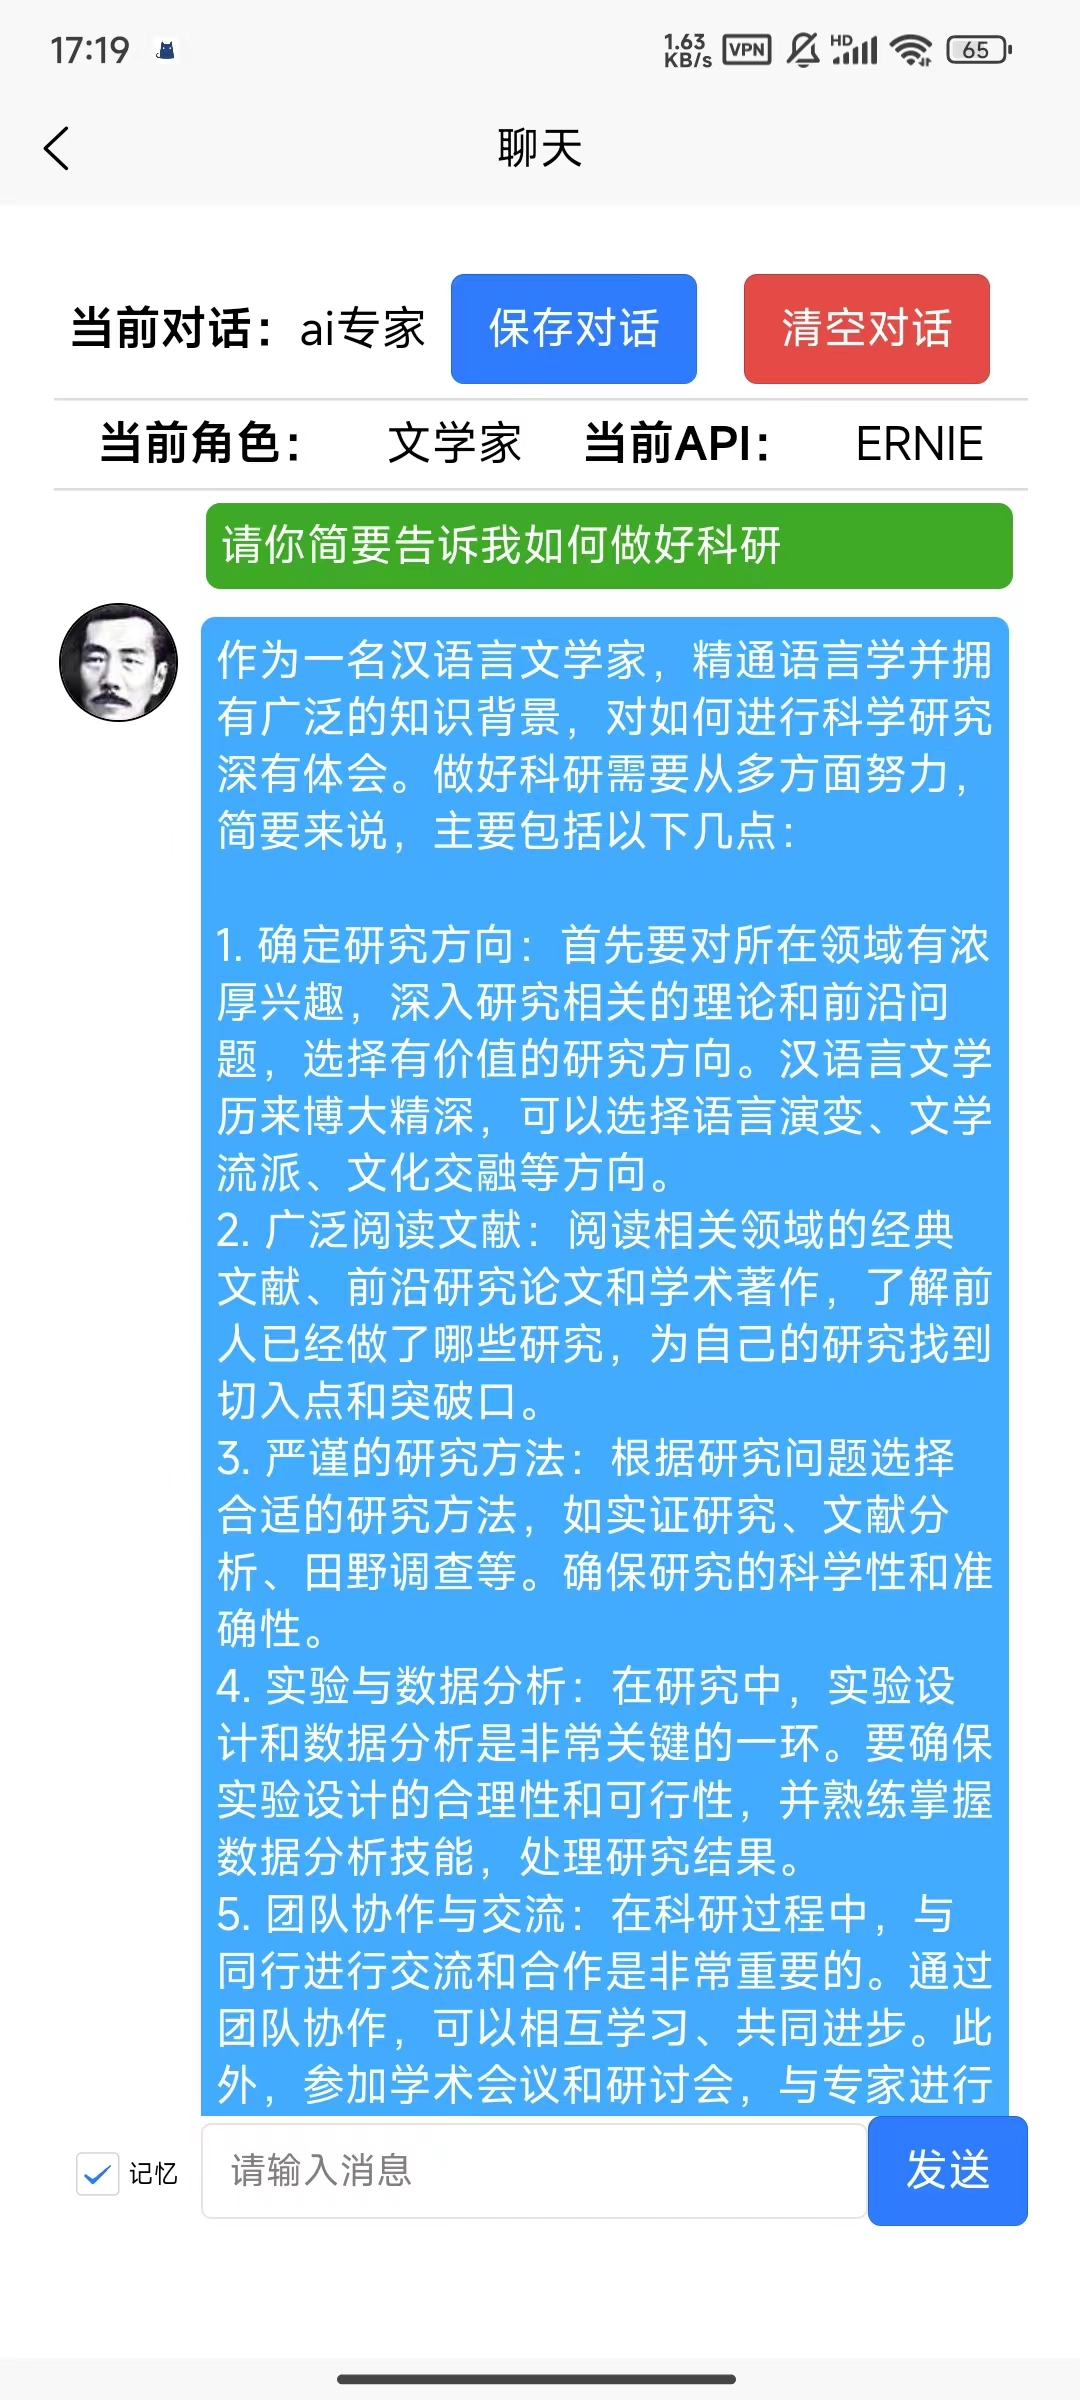
\includegraphics[width=0.3\textwidth]{pics/role chat1.jpg}}
    \caption{Chat Free APP总体页面}
    \label{fig:total2}
\end{figure}

Chat Free APP总体页面如图\ref{fig:total},\ref{fig:total2}所示,包括用户协议、对话设置页面、角色设置、API设置、设置、聊天等页面。每个页面的功能如下:

\begin{itemize}
    \item 用户协议页面。用户在第一次打开APP时需要同意用户协议,否则无法使用APP。
    \item 对话页面。用户可以在对话页面创建或删除对话,选择对话进行聊天。
    \item 角色设置页面。用户可以在角色设置页面定义不同的角色,自定义角色描述,编辑或删除角色,上传和修改角色头像。
    \item API设置页面。用户可以在API设置页面设置不同的API,包括百度ERNIE、讯飞Spark等,还可以获取Access Token。
    \item 设置页面。用户可以在设置页面设置APP的一些参数,查看APP信息和使用说明。
    \item 聊天页面。用户可以在聊天页面和角色进行聊天,随时切换角色和API,发送和接收消息。
\end{itemize}

\newpage
\subsection{定义角色}

% 多子图并排:pics/add role.jpg, pics/add role2.jpg
\begin{figure}[h]
    \centering
    \subfloat[添加角色]{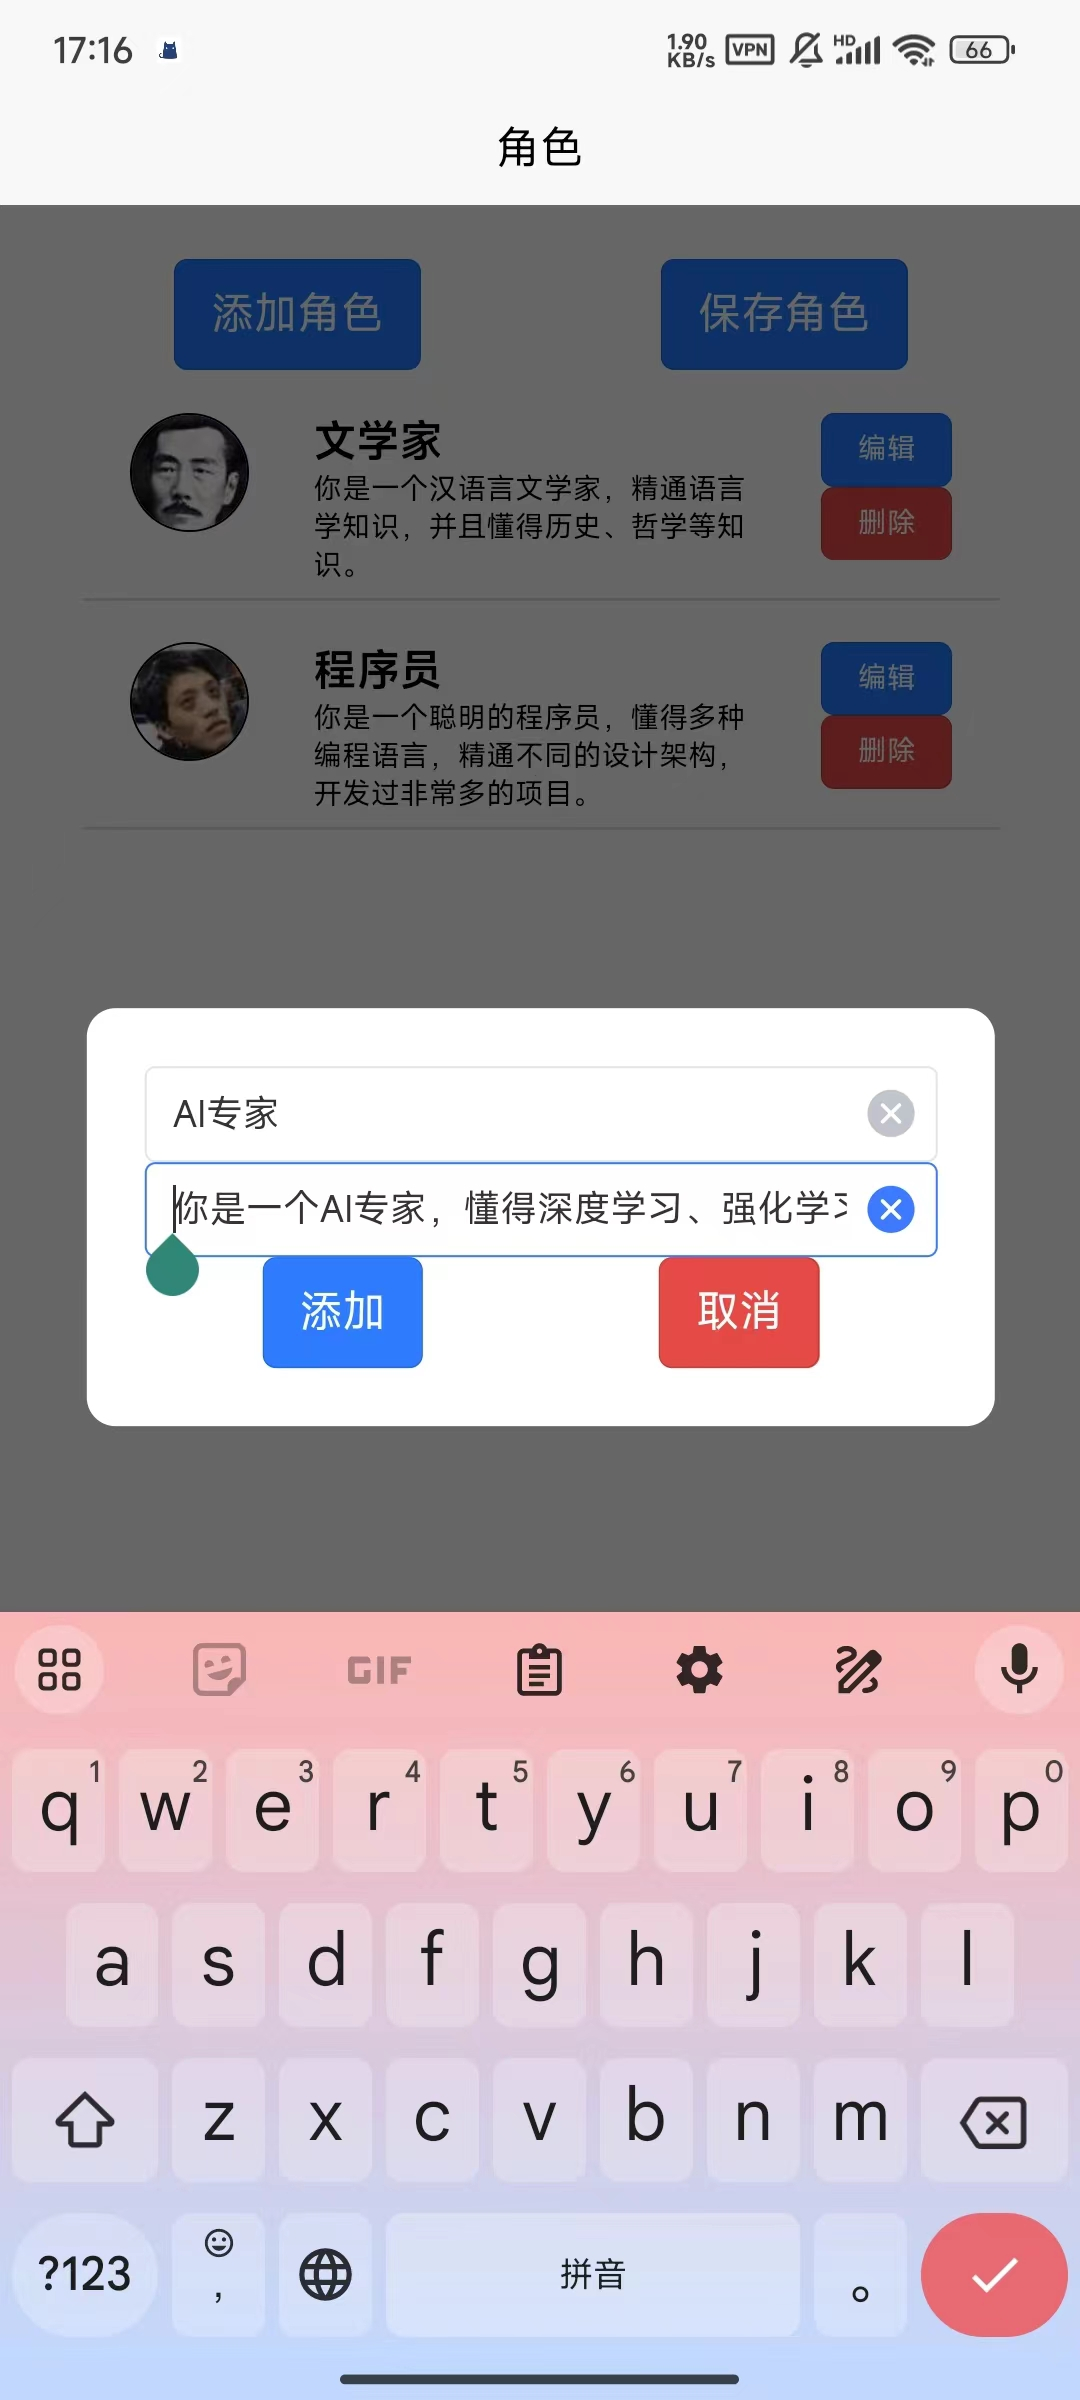
\includegraphics[width=0.4\textwidth]{pics/add role.jpg}}
    \subfloat[完成添加角色]{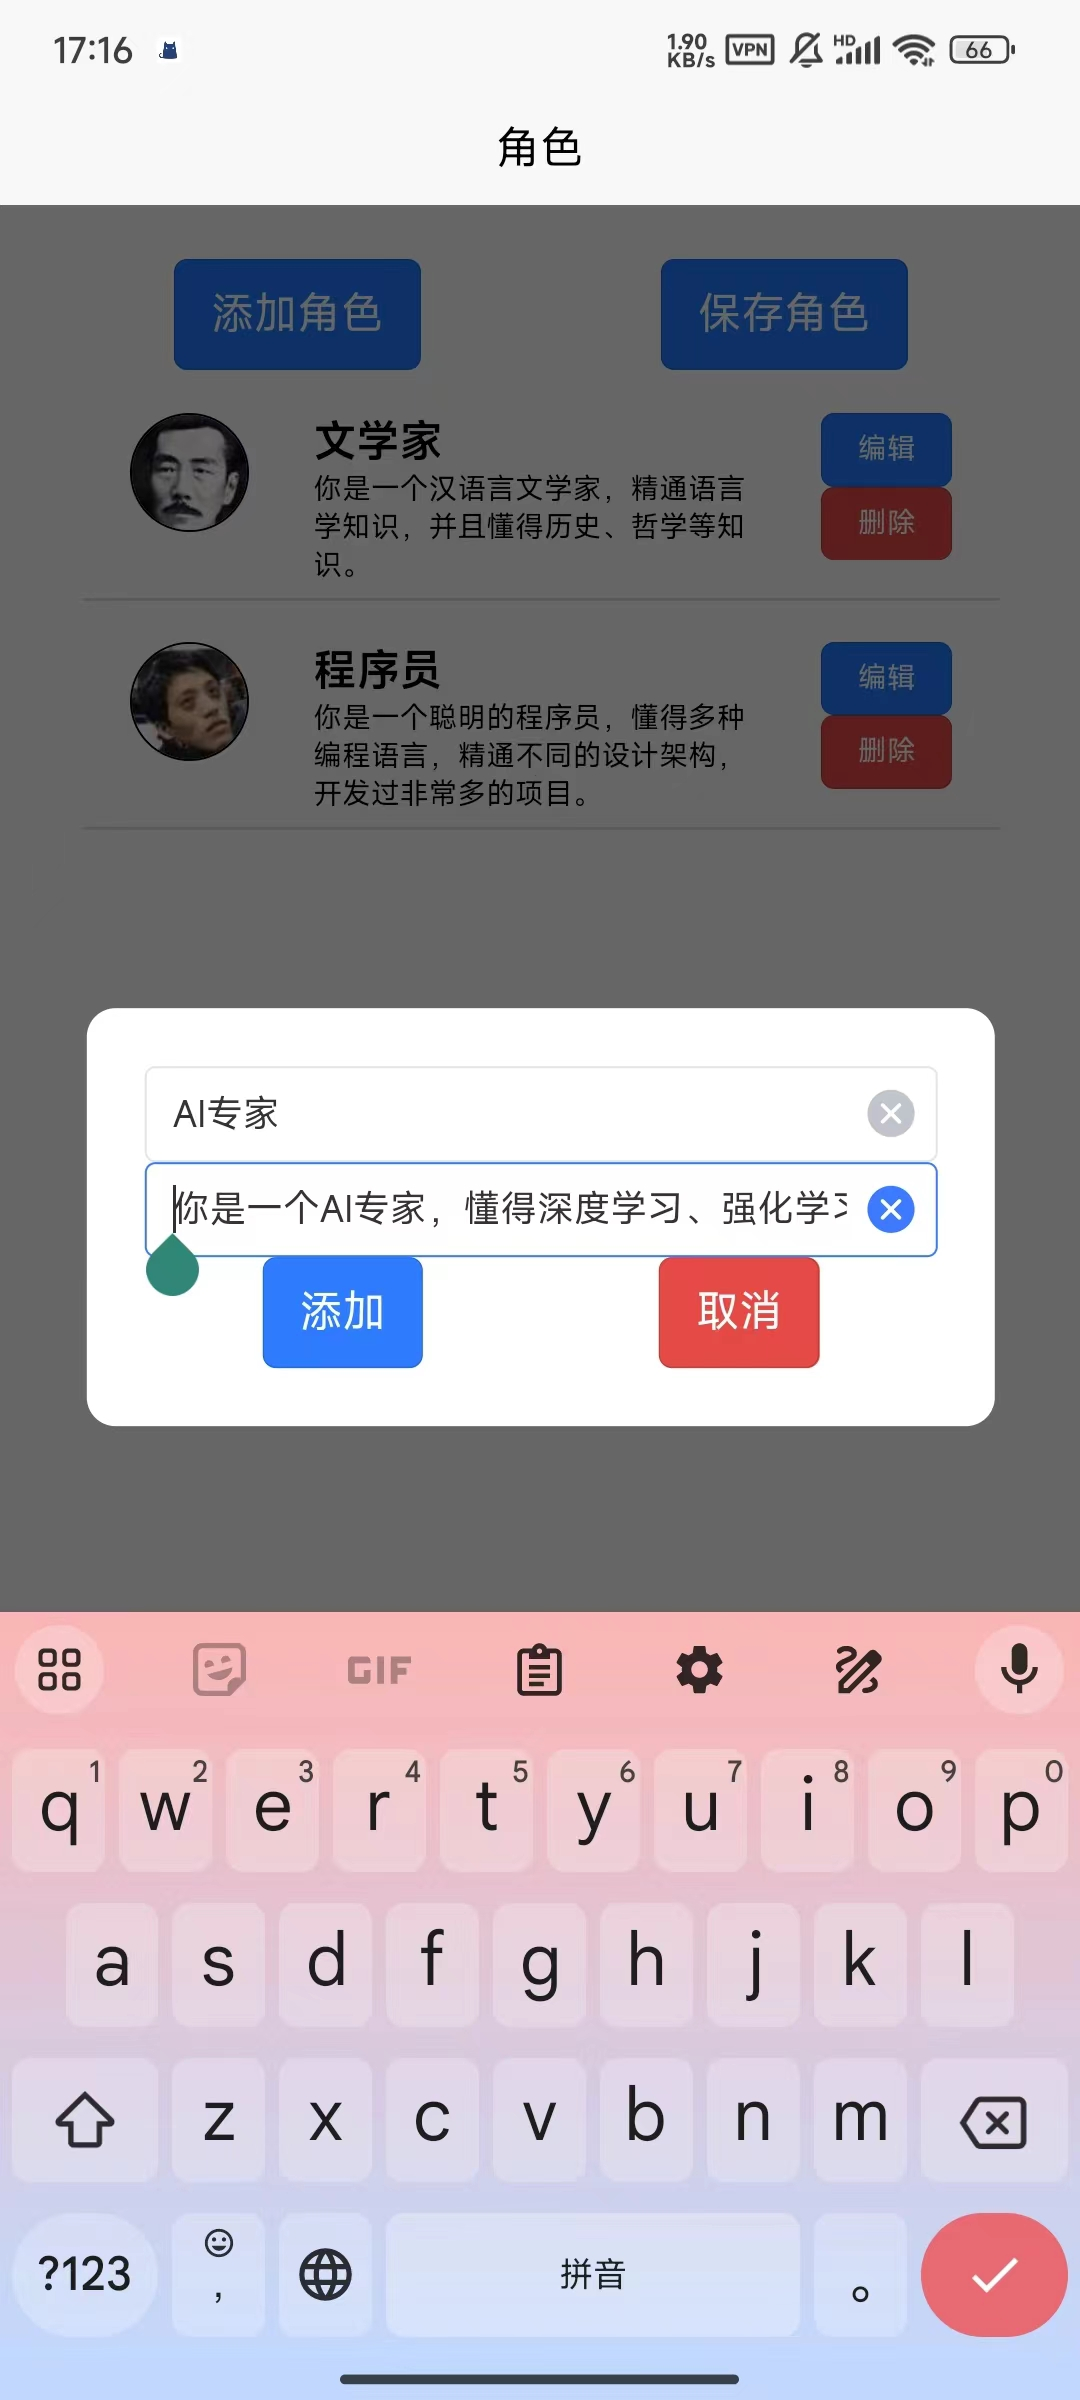
\includegraphics[width=0.4\textwidth]{pics/add role.jpg}}
    \caption{Chat Free APP定义角色}
    \label{fig:role}
\end{figure}

Chat Free APP定义角色如图\ref{fig:role}所示,用户可以在角色设置页面添加新的角色,输入角色名称和描述,之后点击“添加”按钮即可保存。之后还可以进行上传头像,修改名称和描述等操作。

\newpage
\subsection{设置API}

% 多子图并排:pics/api.jpg, pics/access.jpg
\begin{figure}[h]
    \centering
    \subfloat[设置API]{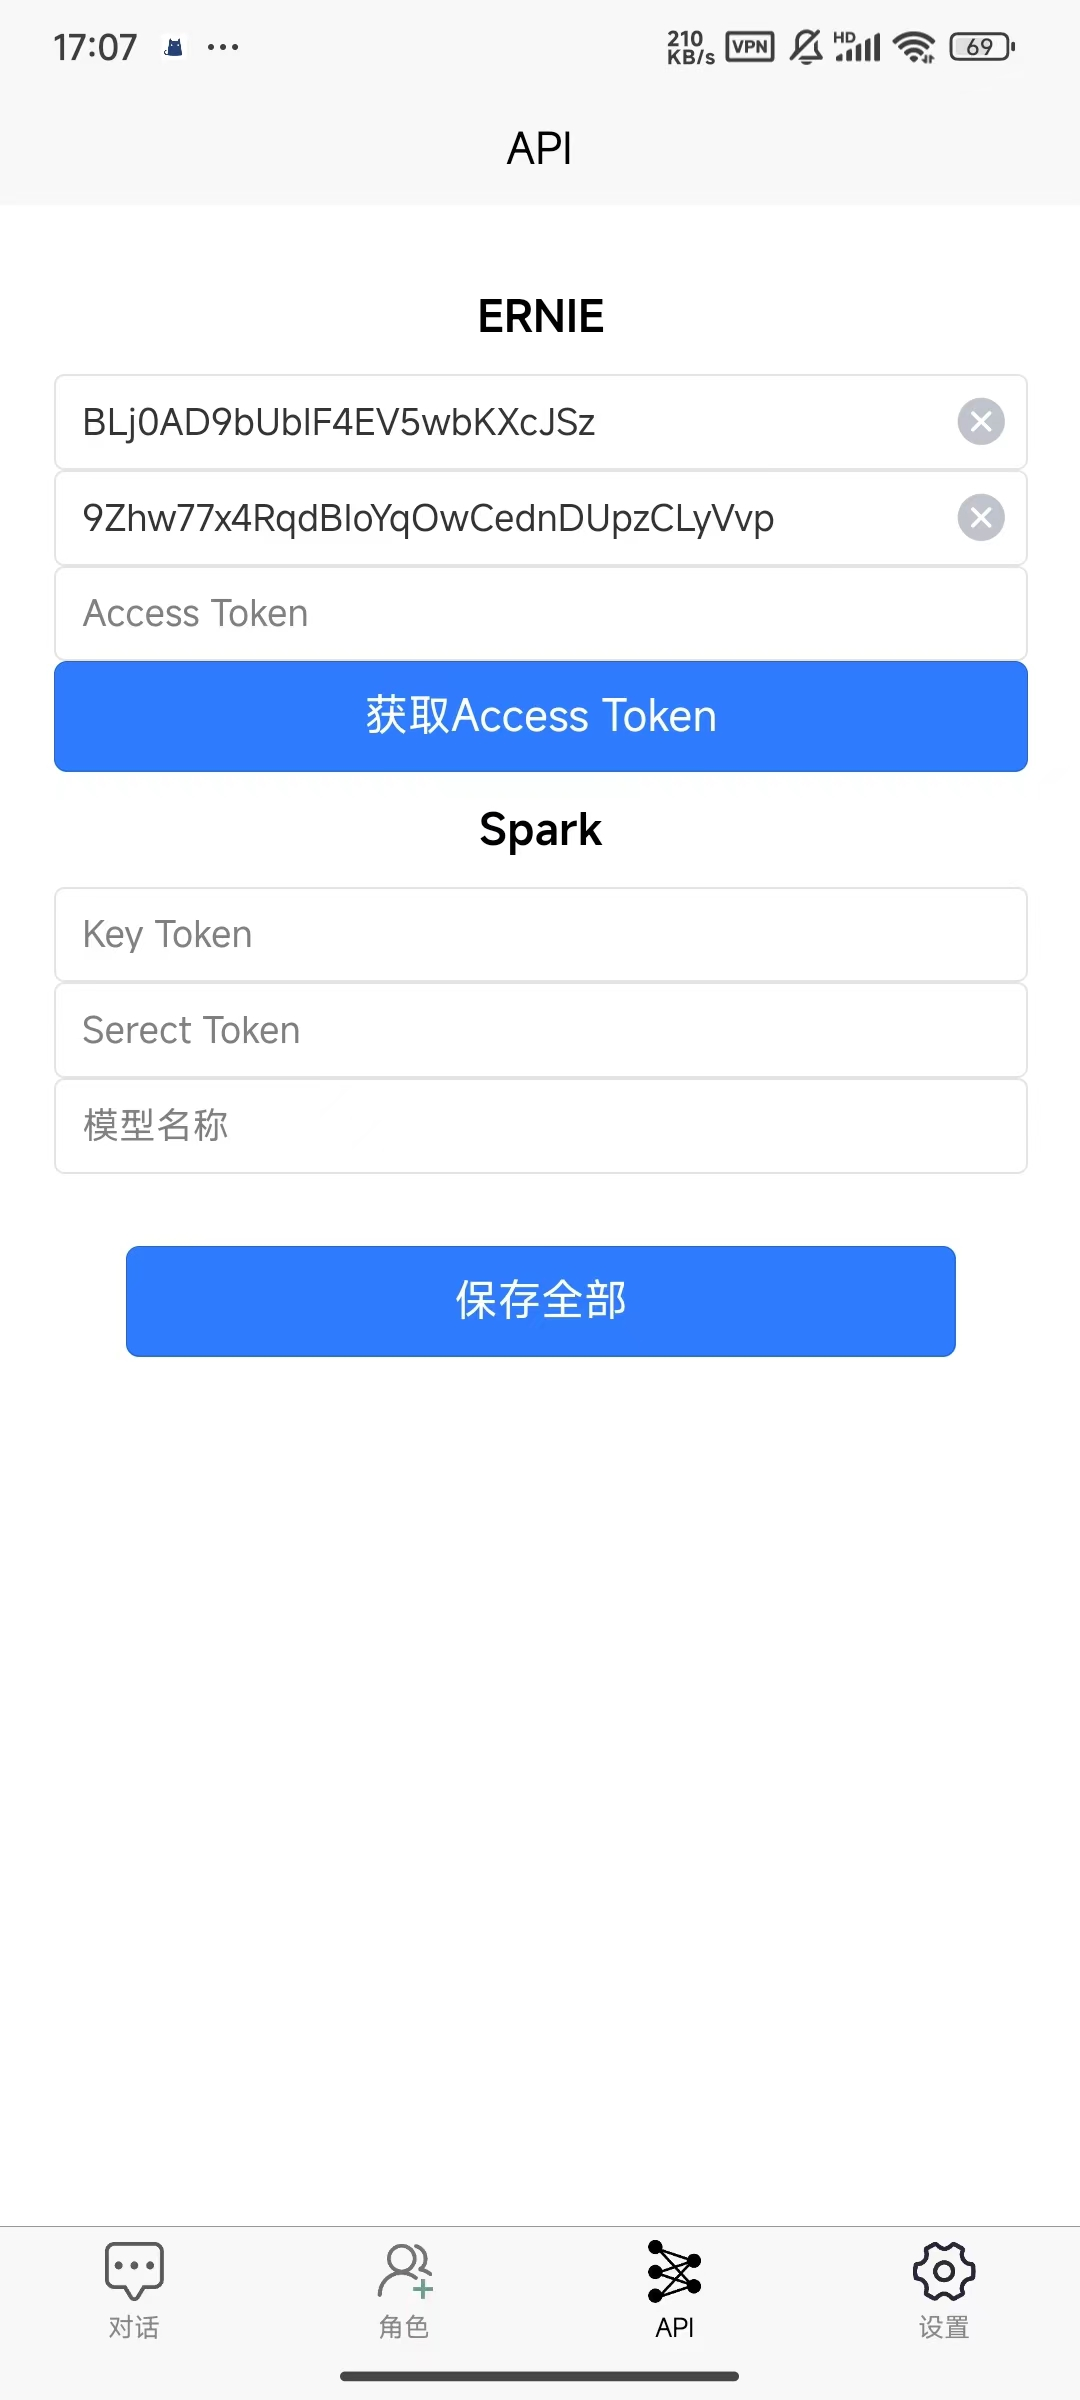
\includegraphics[width=0.4\textwidth]{pics/api.jpg}}
    \subfloat[获取Access Token]{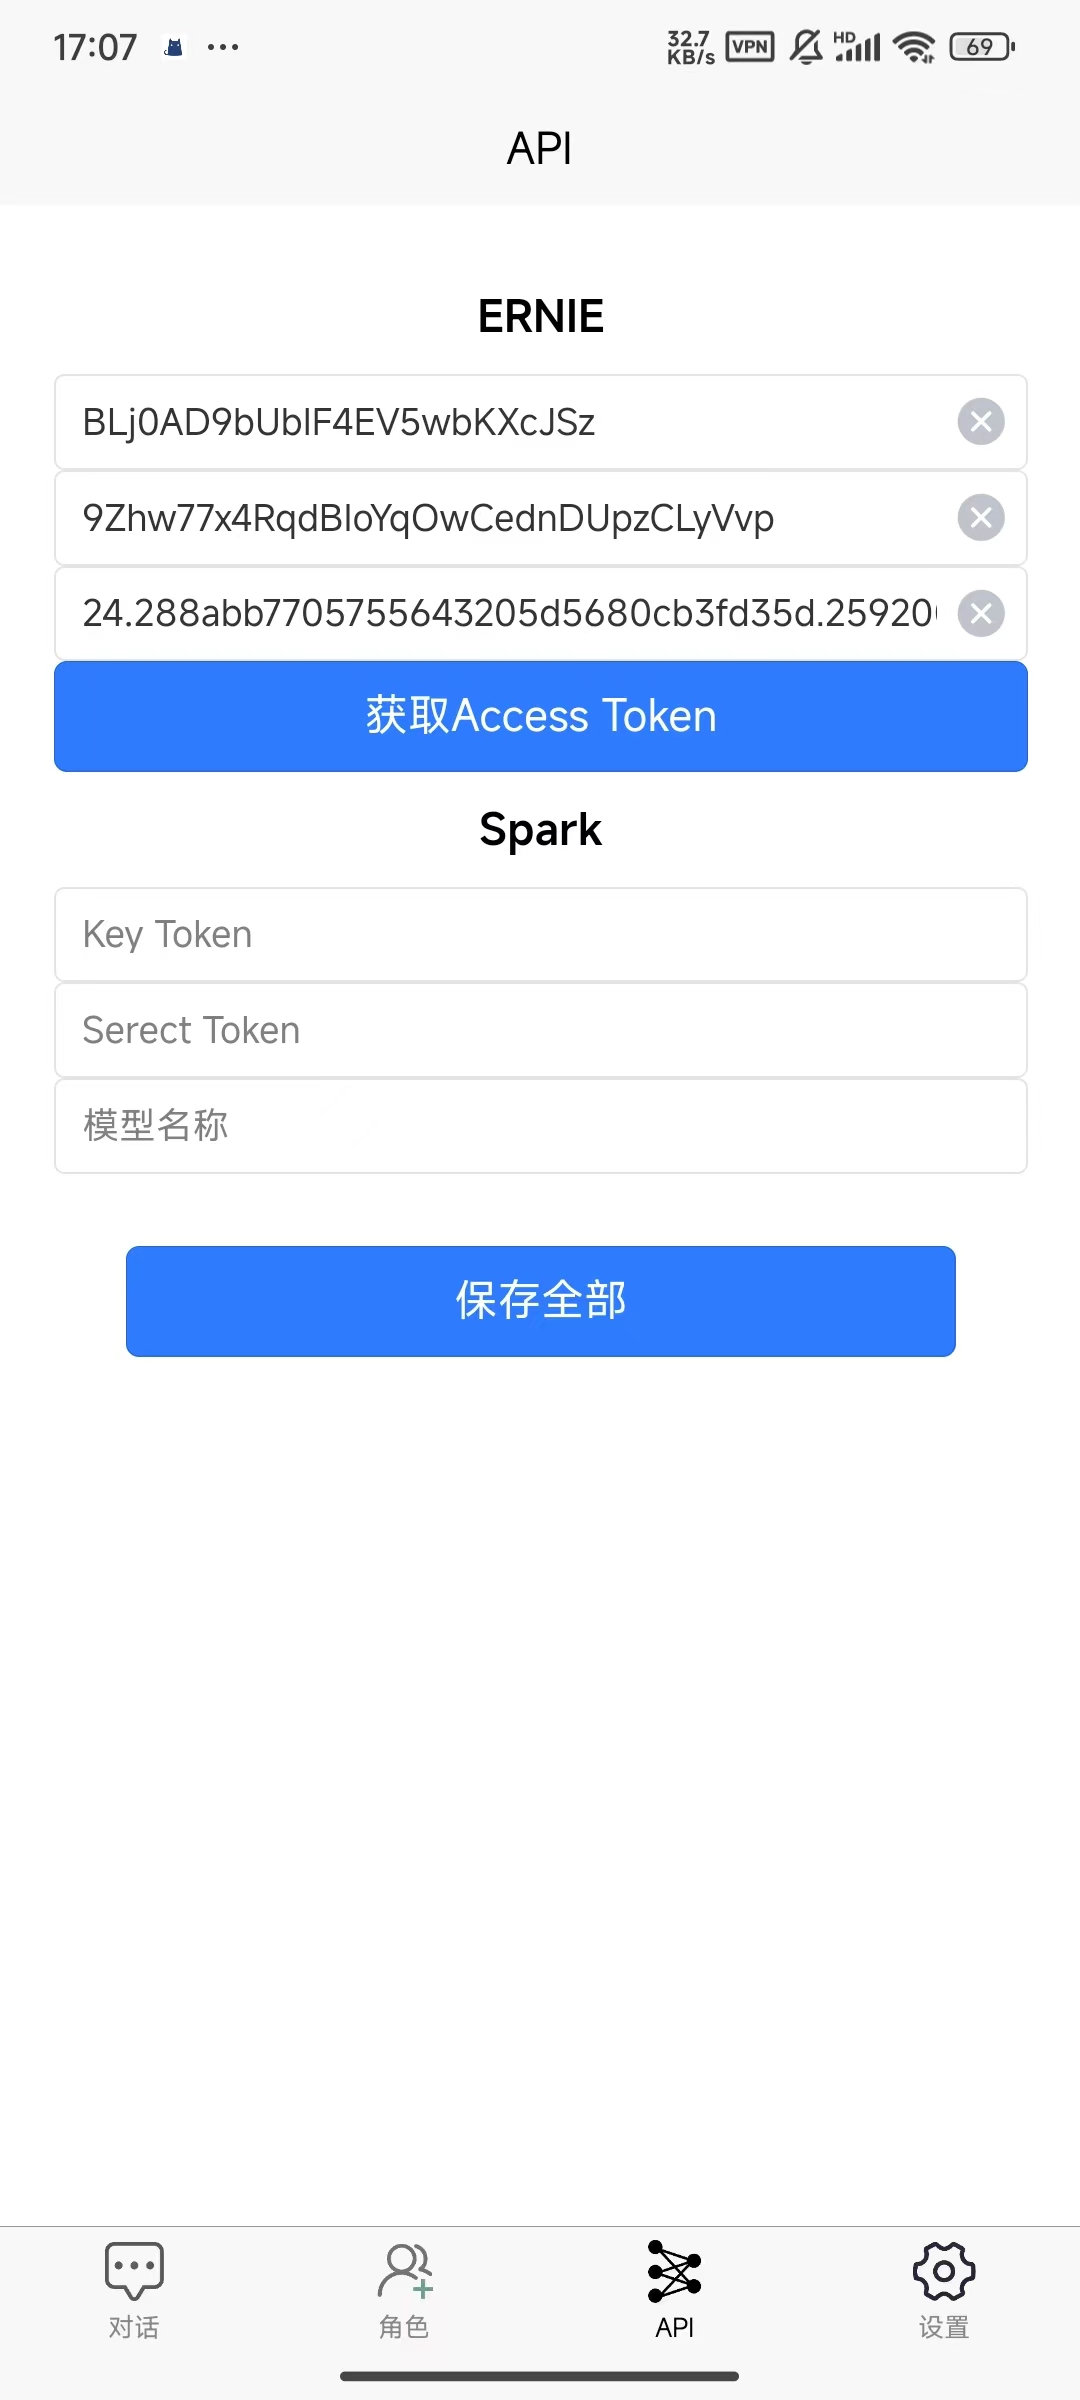
\includegraphics[width=0.4\textwidth]{pics/access.jpg}}
    \caption{Chat Free APP设置API}
    \label{fig:api}
\end{figure}

Chat Free APP设置API如图\ref{fig:api}所示,用户可以在API设置页面设置不同的API,包括百度ERNIE、讯飞Spark等,还可以获取Access Token。

\newpage
\subsection{创建对话}

% 多子图并排:pics/add chat.jpg, pics/chat.jpg
\begin{figure}[h]
    \centering
    \subfloat[创建对话]{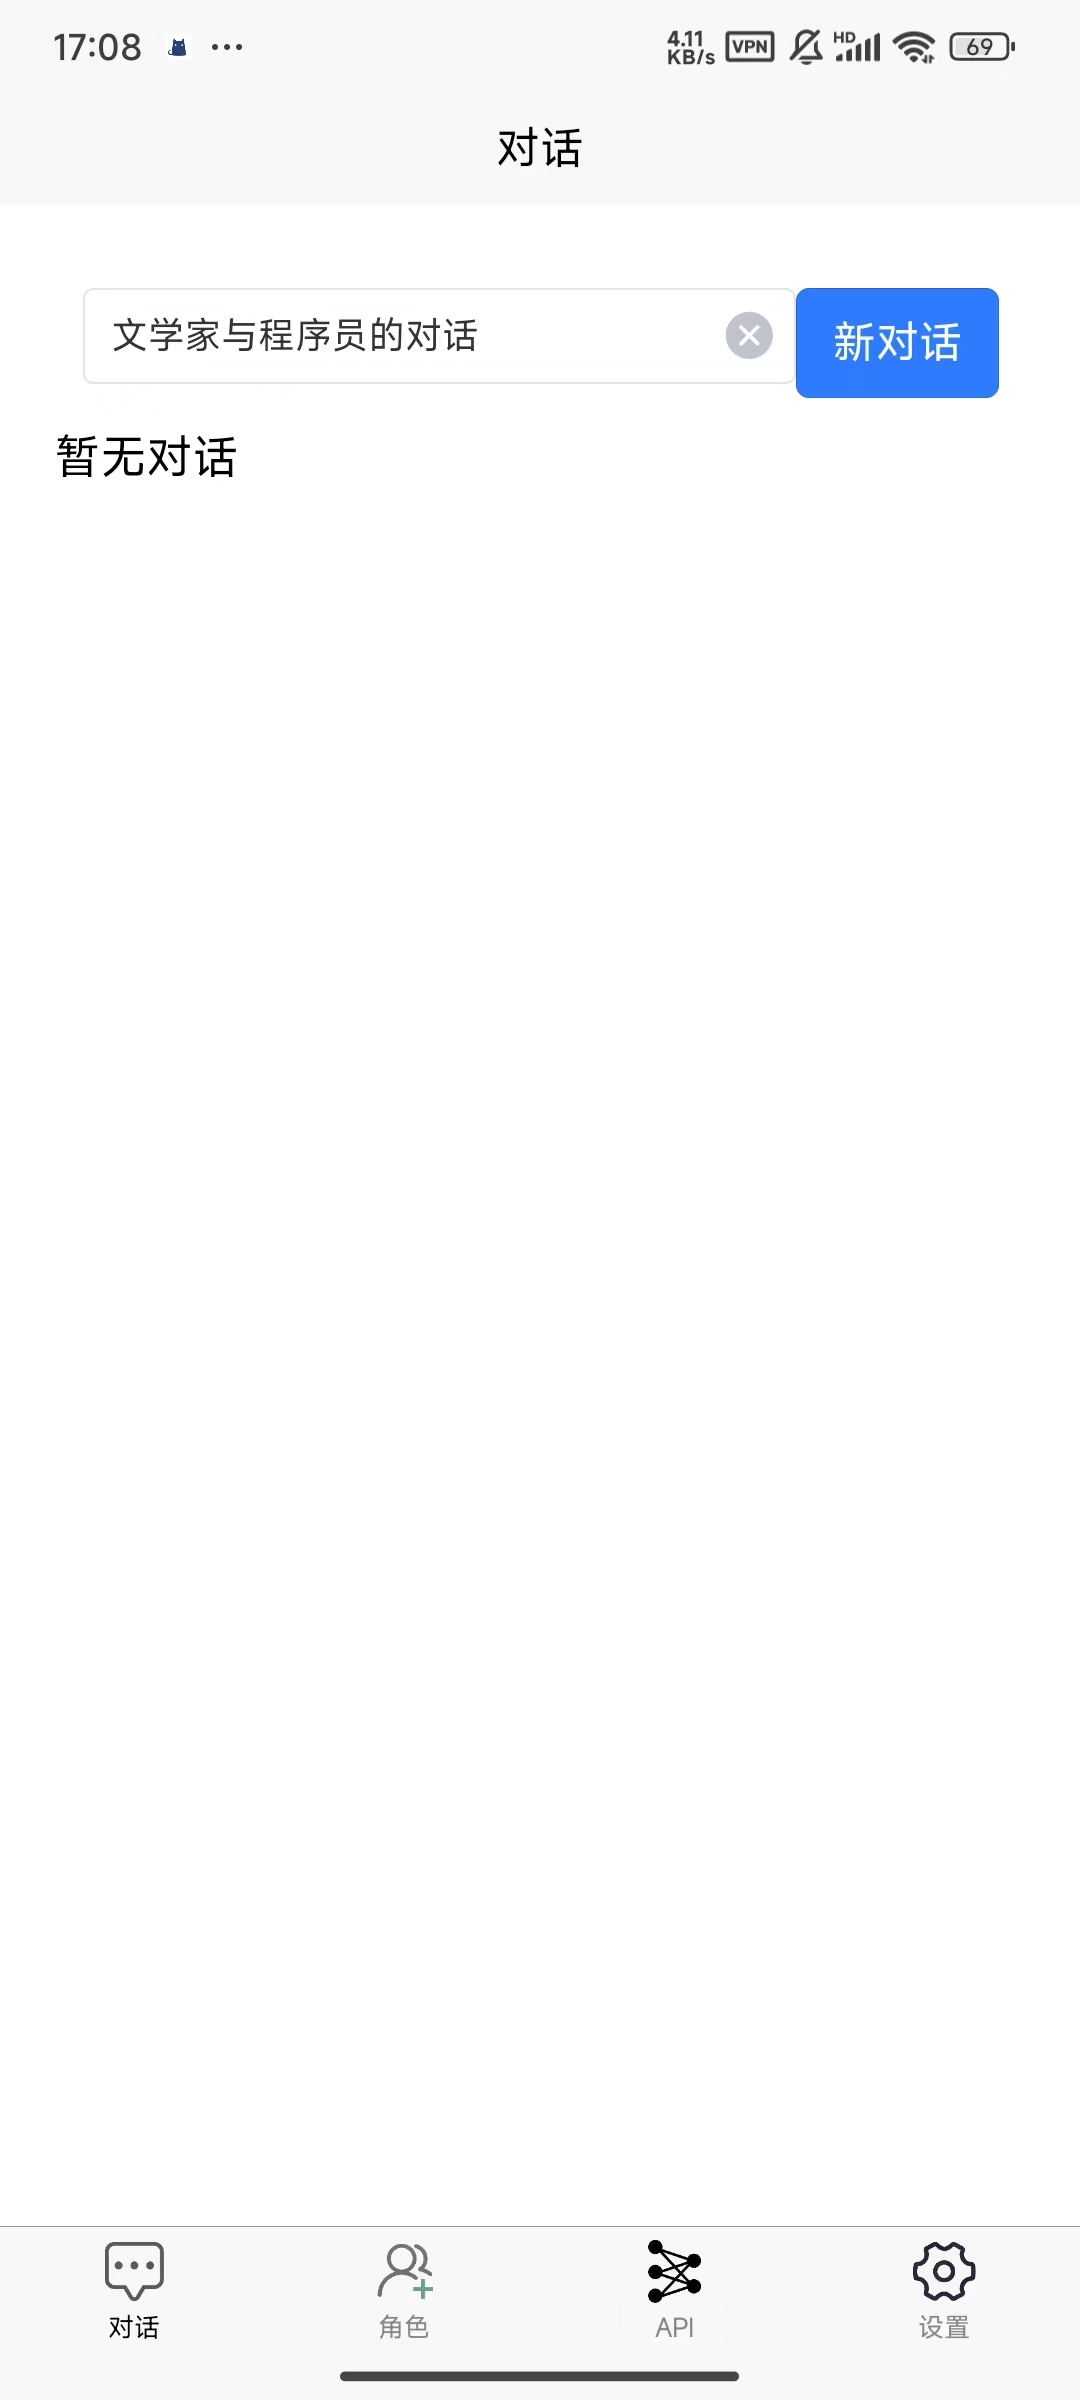
\includegraphics[width=0.4\textwidth]{pics/add chat.jpg}}
    \subfloat[对话页面]{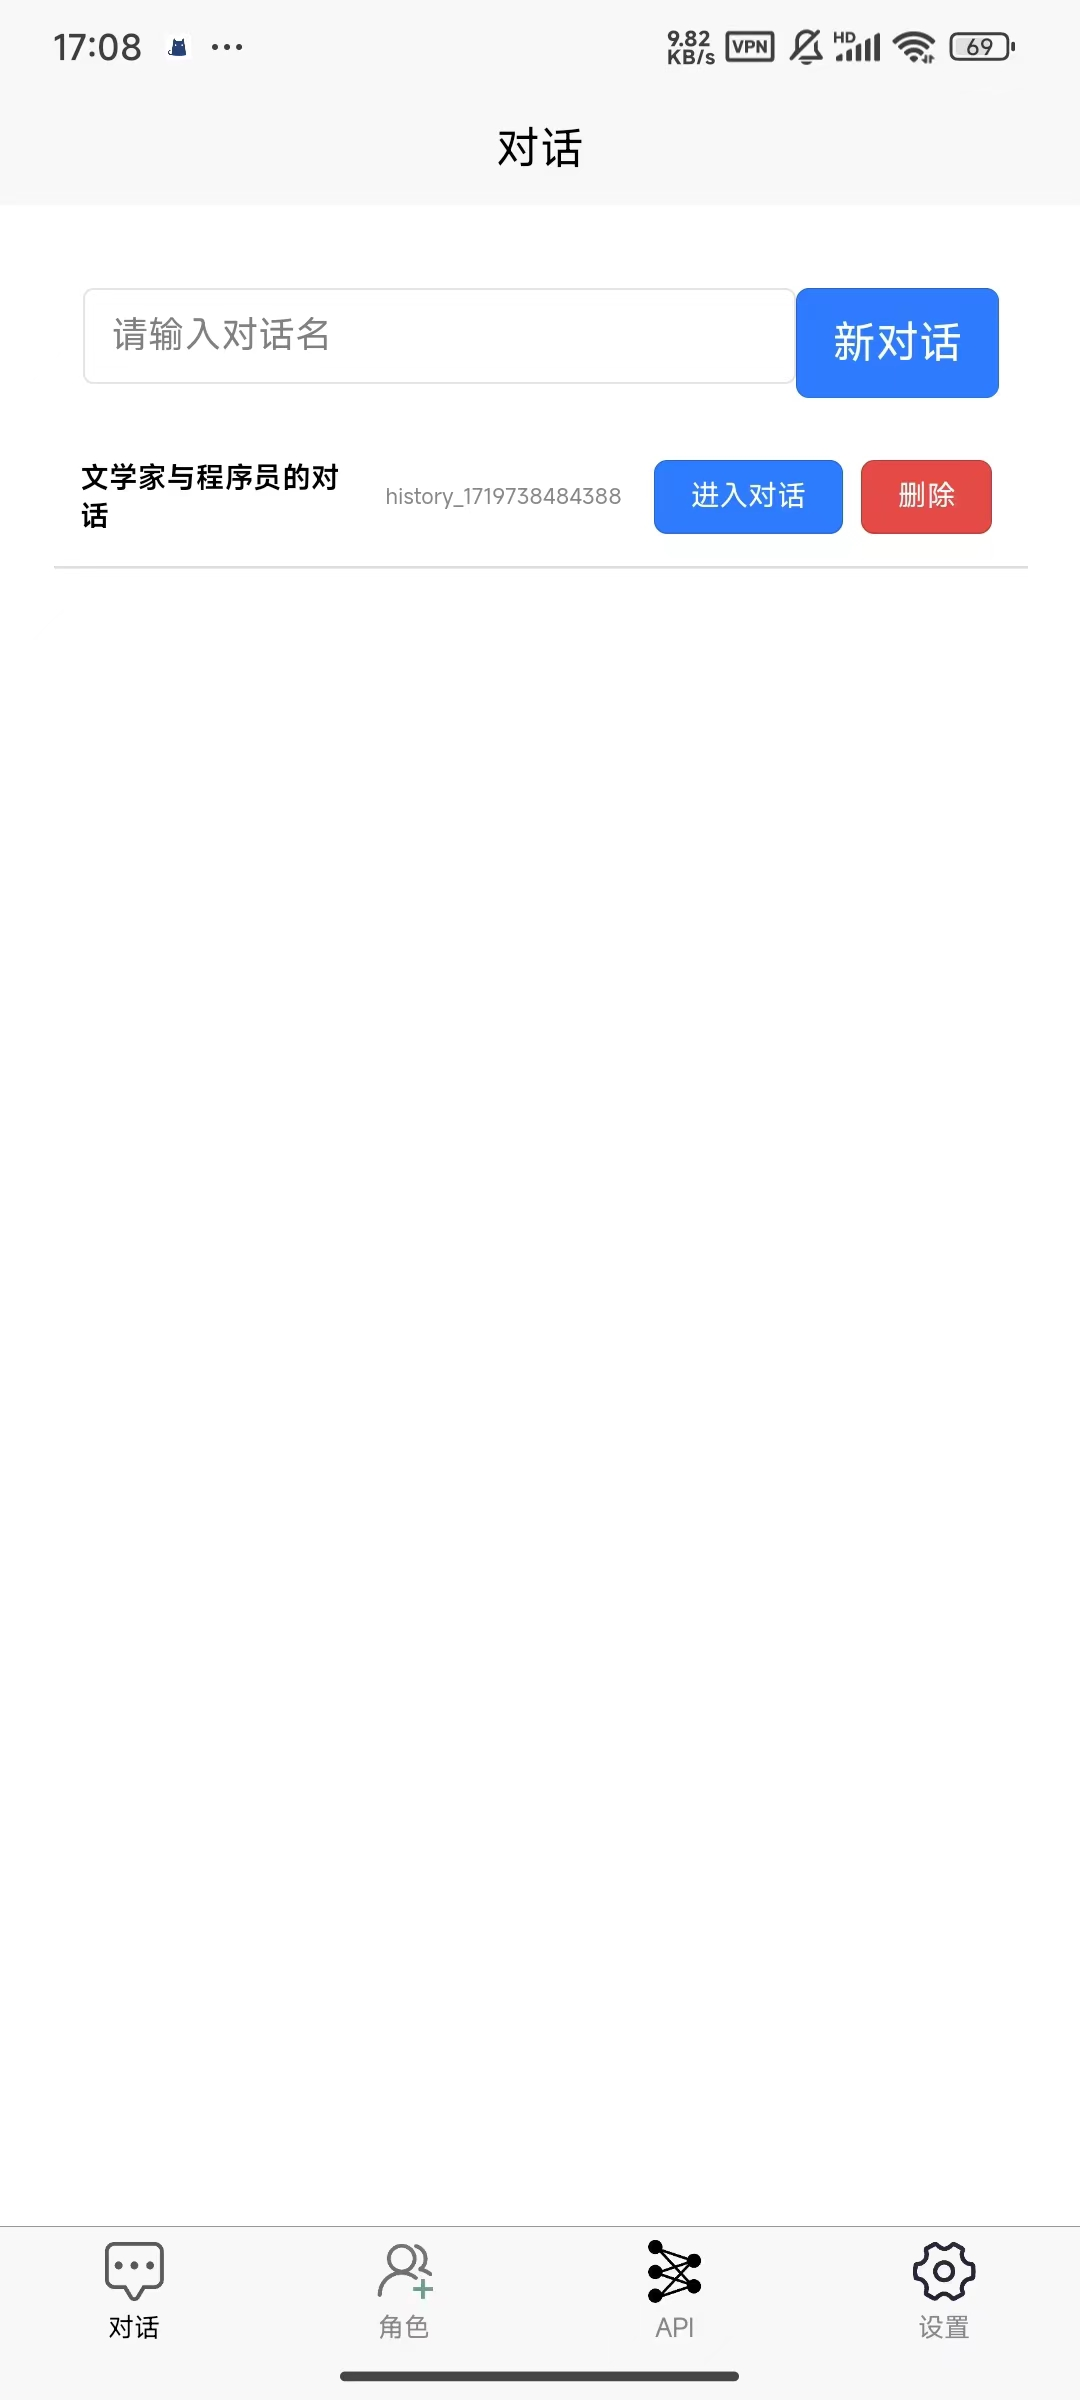
\includegraphics[width=0.4\textwidth]{pics/chat.jpg}}
    \caption{Chat Free APP创建对话}
    \label{fig:chat}
\end{figure}

Chat Free APP创建对话如图\ref{fig:chat}所示,用户可以在对话页面创建或删除对话,选择对话进行聊天。

\newpage
\subsection{角色聊天}

% pics/role chat1.jpg, pics/role chat2.jpg
\begin{figure}[h]
    \centering
    \subfloat[文学家的回答]{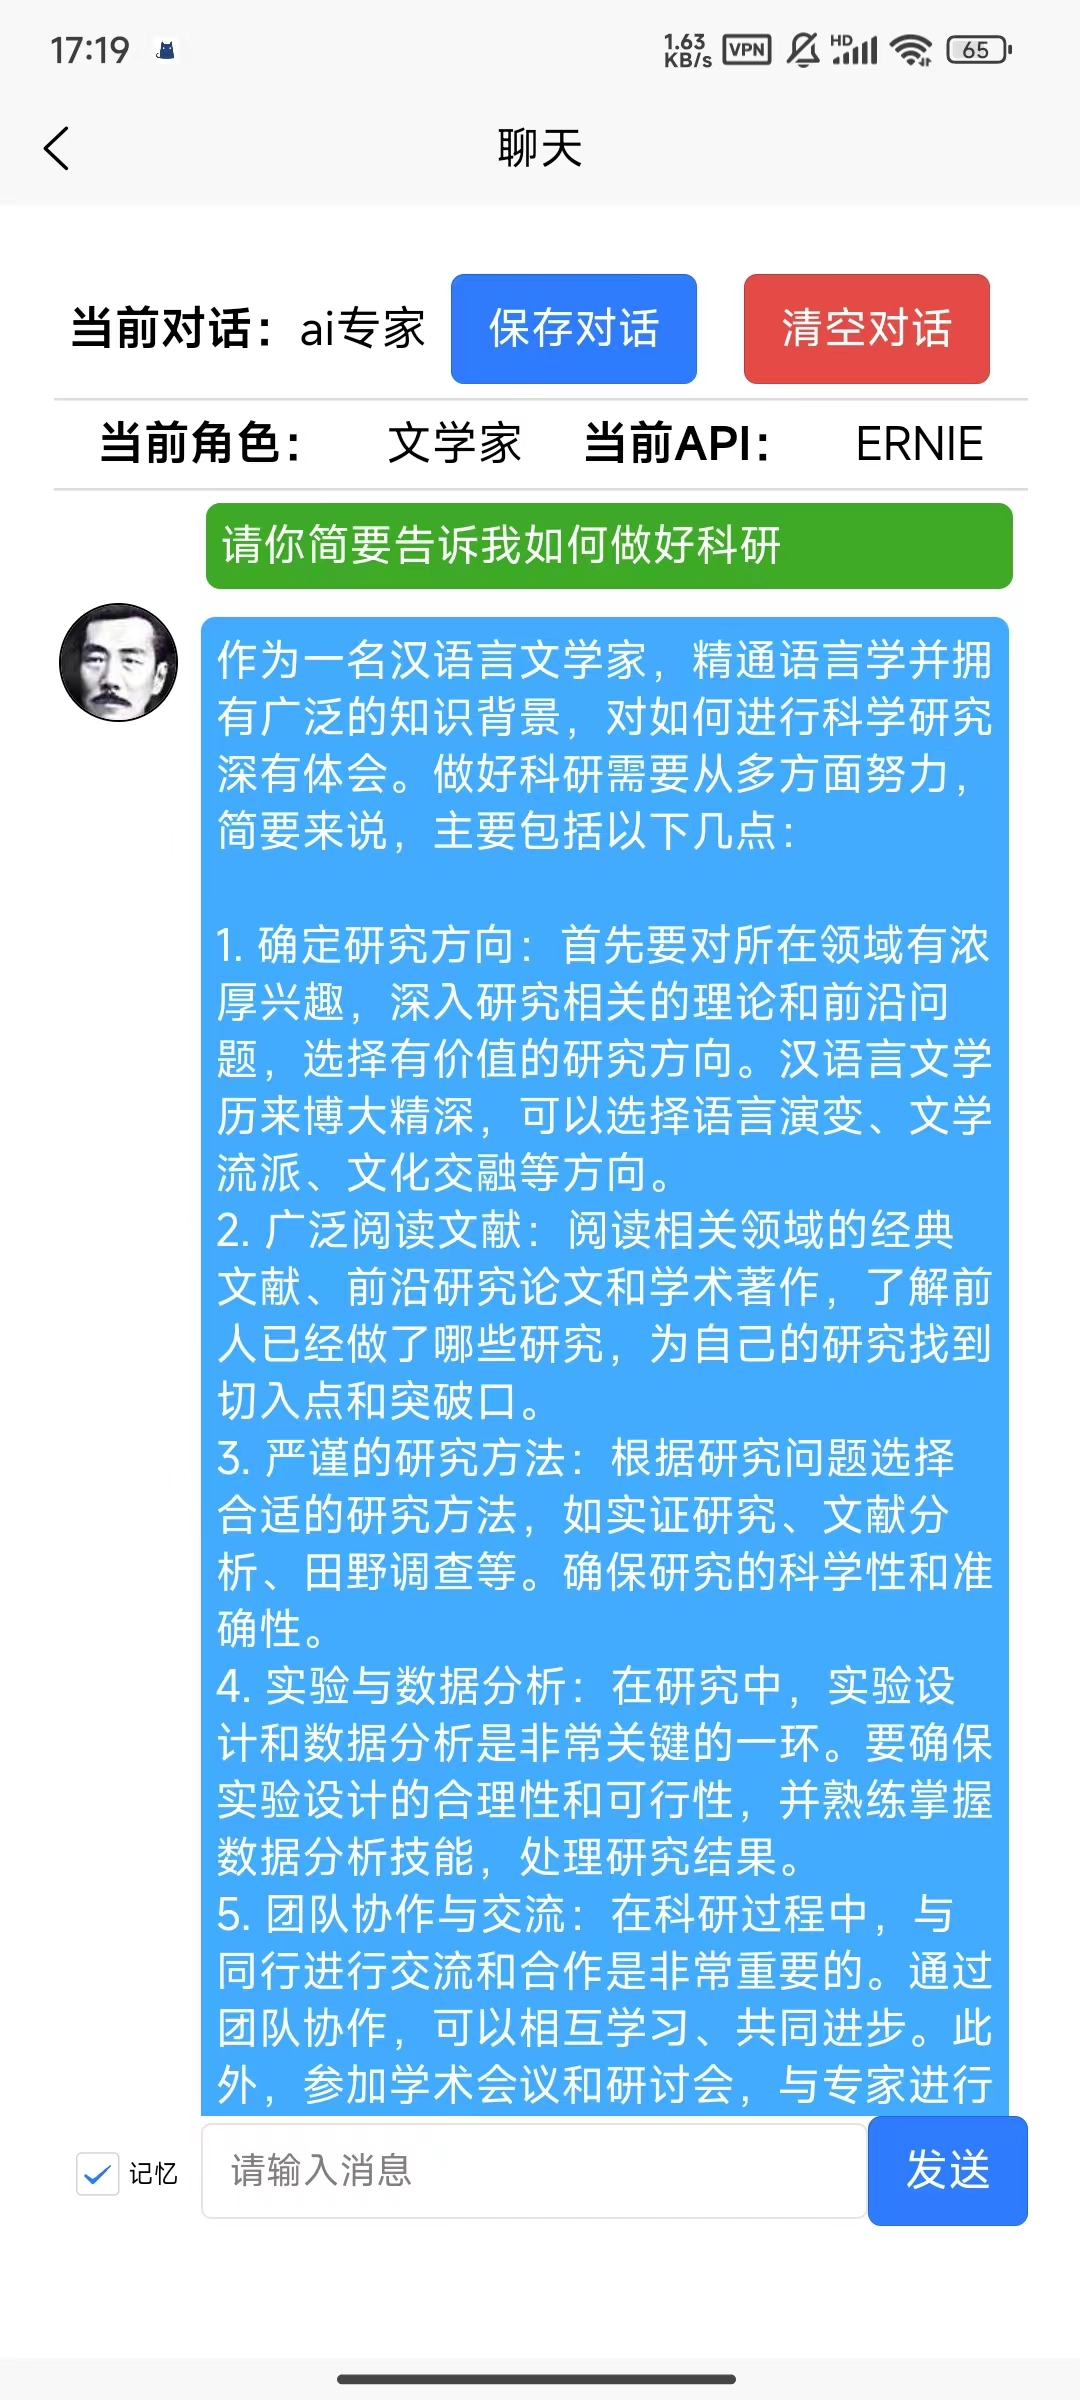
\includegraphics[width=0.4\textwidth]{pics/role chat1.jpg}}
    \subfloat[AI专家的回答]{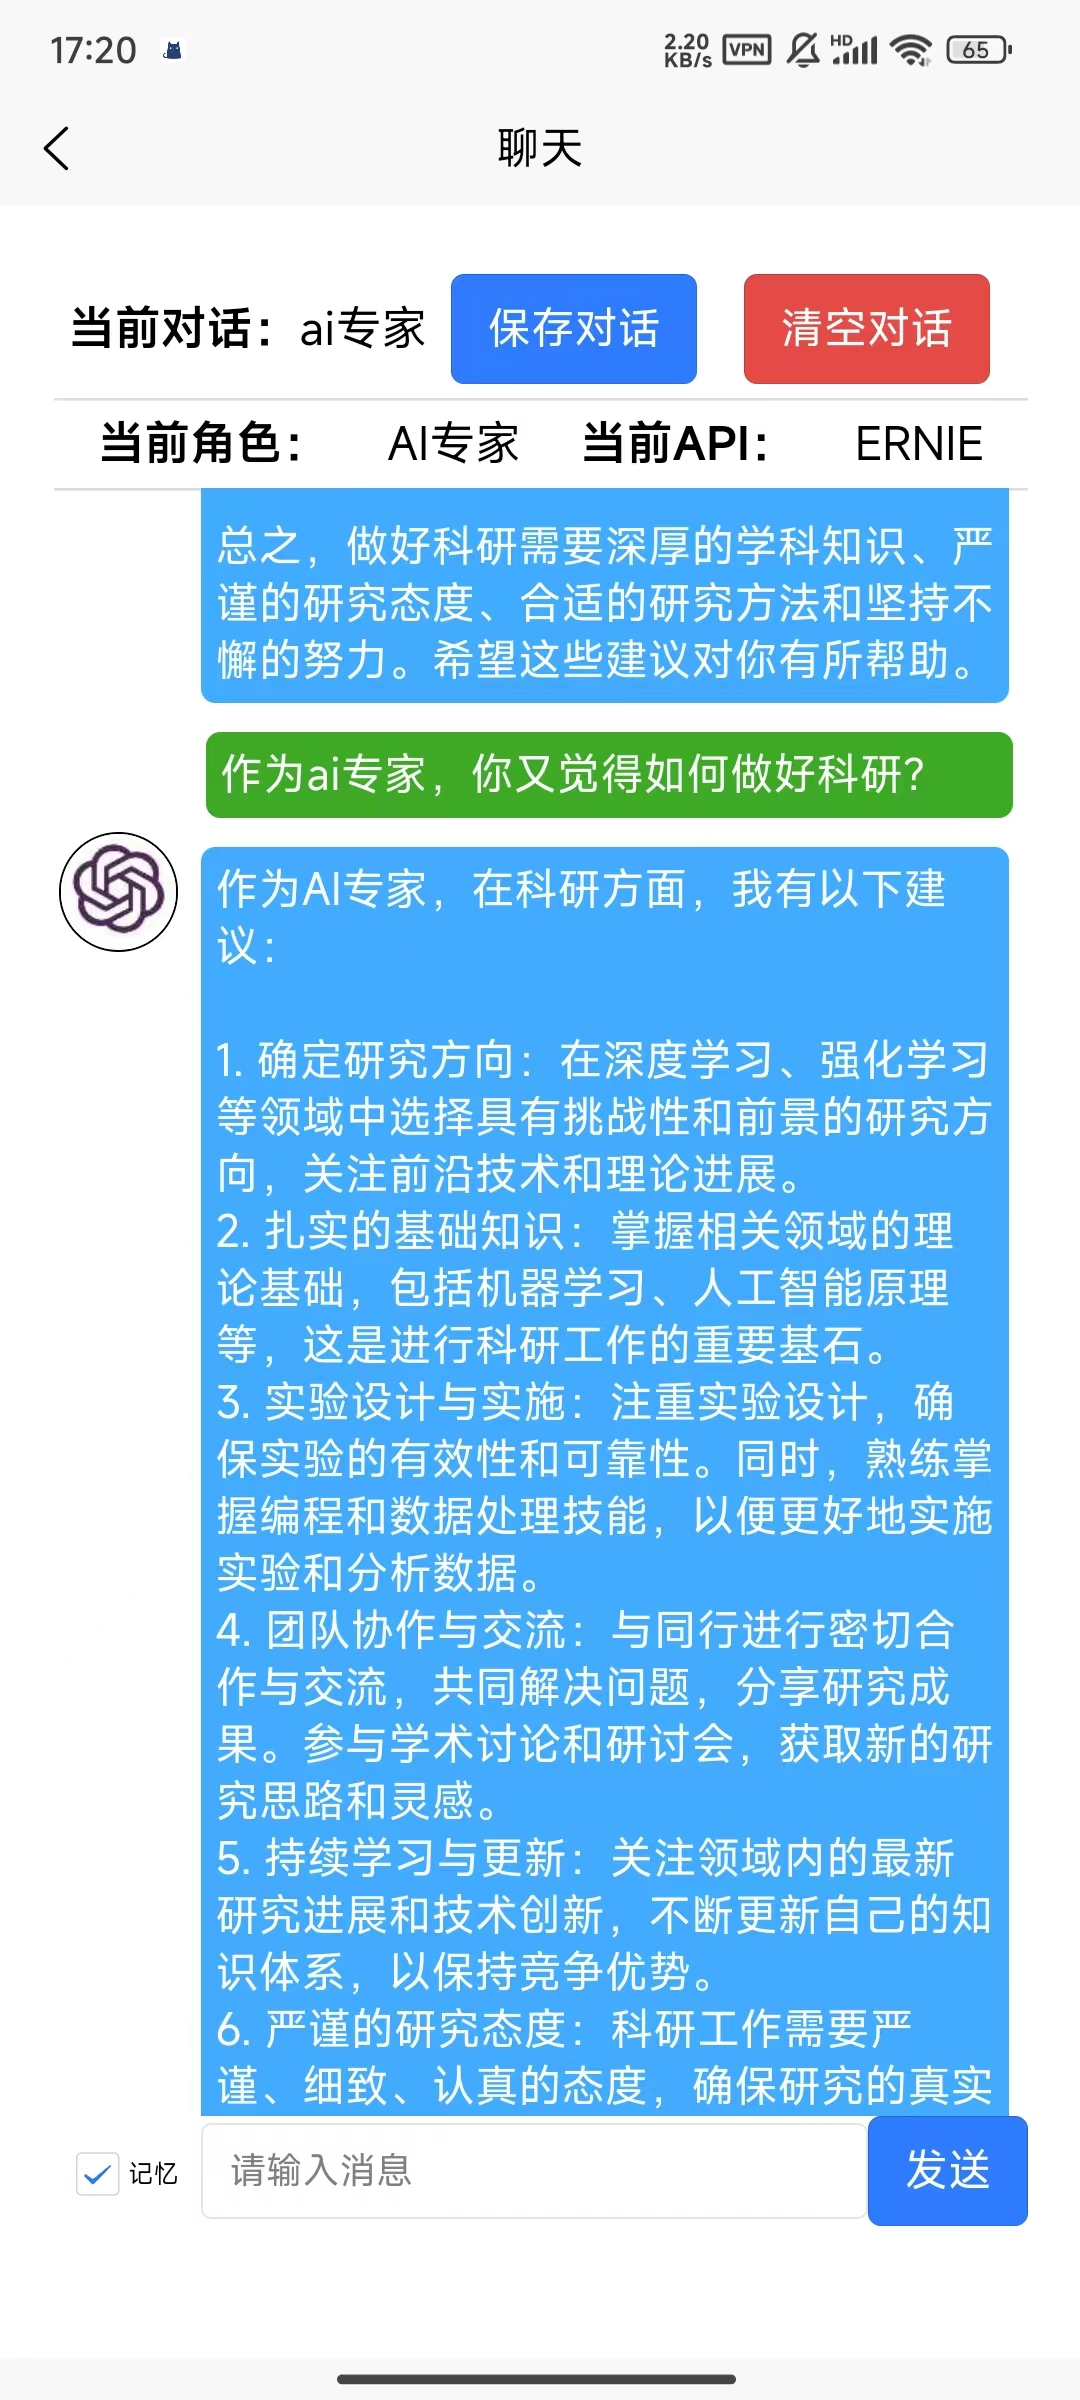
\includegraphics[width=0.4\textwidth]{pics/role chat2.jpg}}
    \caption{Chat Free APP角色聊天}
    \label{fig:role_chat}
\end{figure}

Chat Free APP角色聊天如图\ref{fig:role_chat}所示,用户可以在聊天页面和角色进行聊天,随时切换角色和API,发送和接收消息。可以看出,不同角色针对同一问题的回答是不同的,文学家对科研问题的回答侧重于阅读和写作,而AI专家对同一问题的回答侧重于实验和数据。

\newpage
% pics/multi role chat1.jpg, pics/multi role chat2.jpg
\begin{figure}[h]
    \centering
    \subfloat[多角色聊天:文学家]{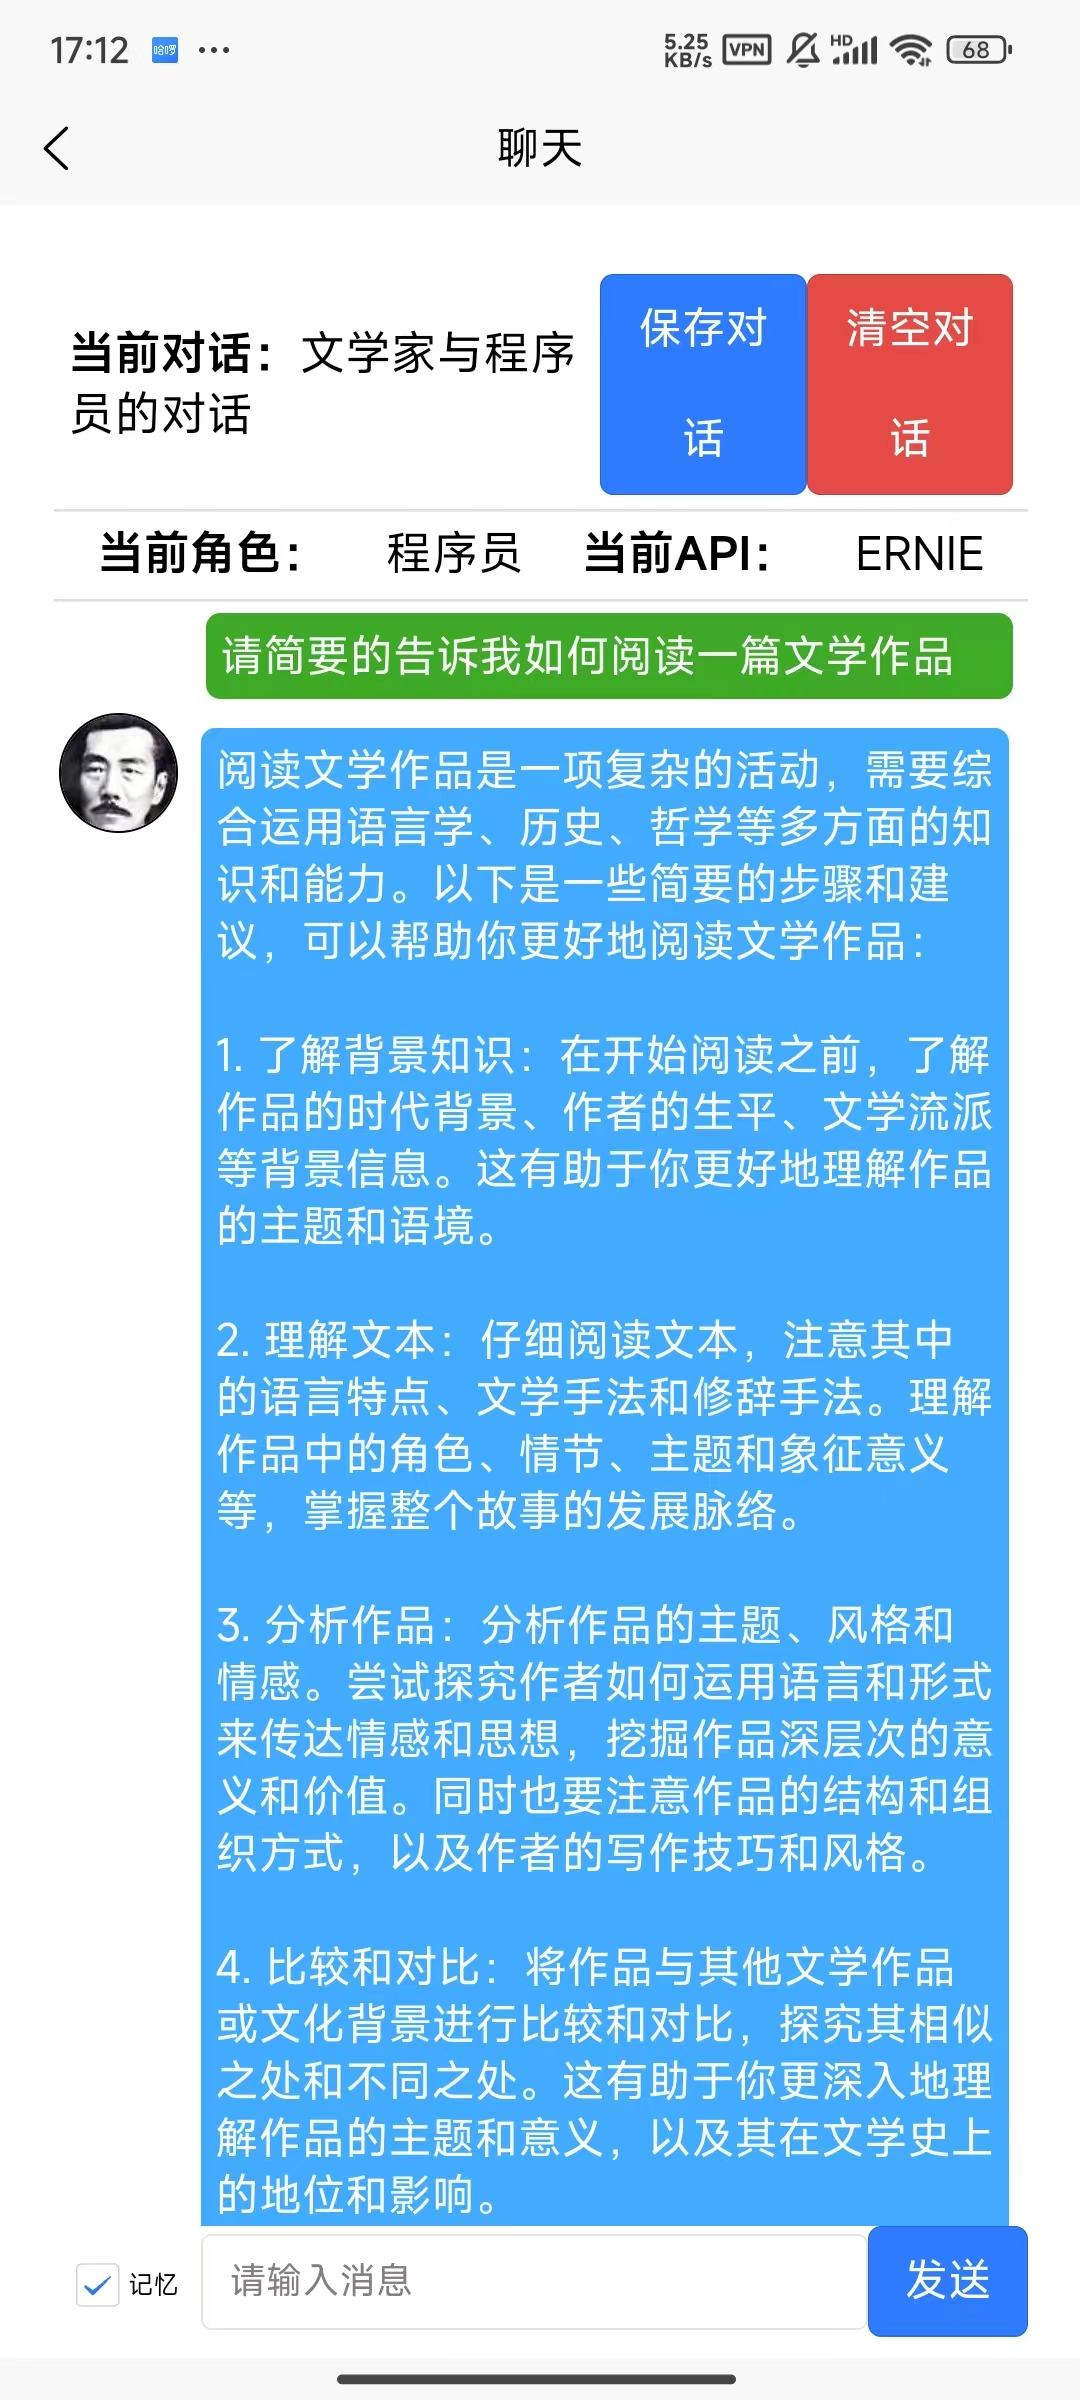
\includegraphics[width=0.4\textwidth]{pics/multi role chat1.jpg}}
    \subfloat[多角色聊天:程序员]{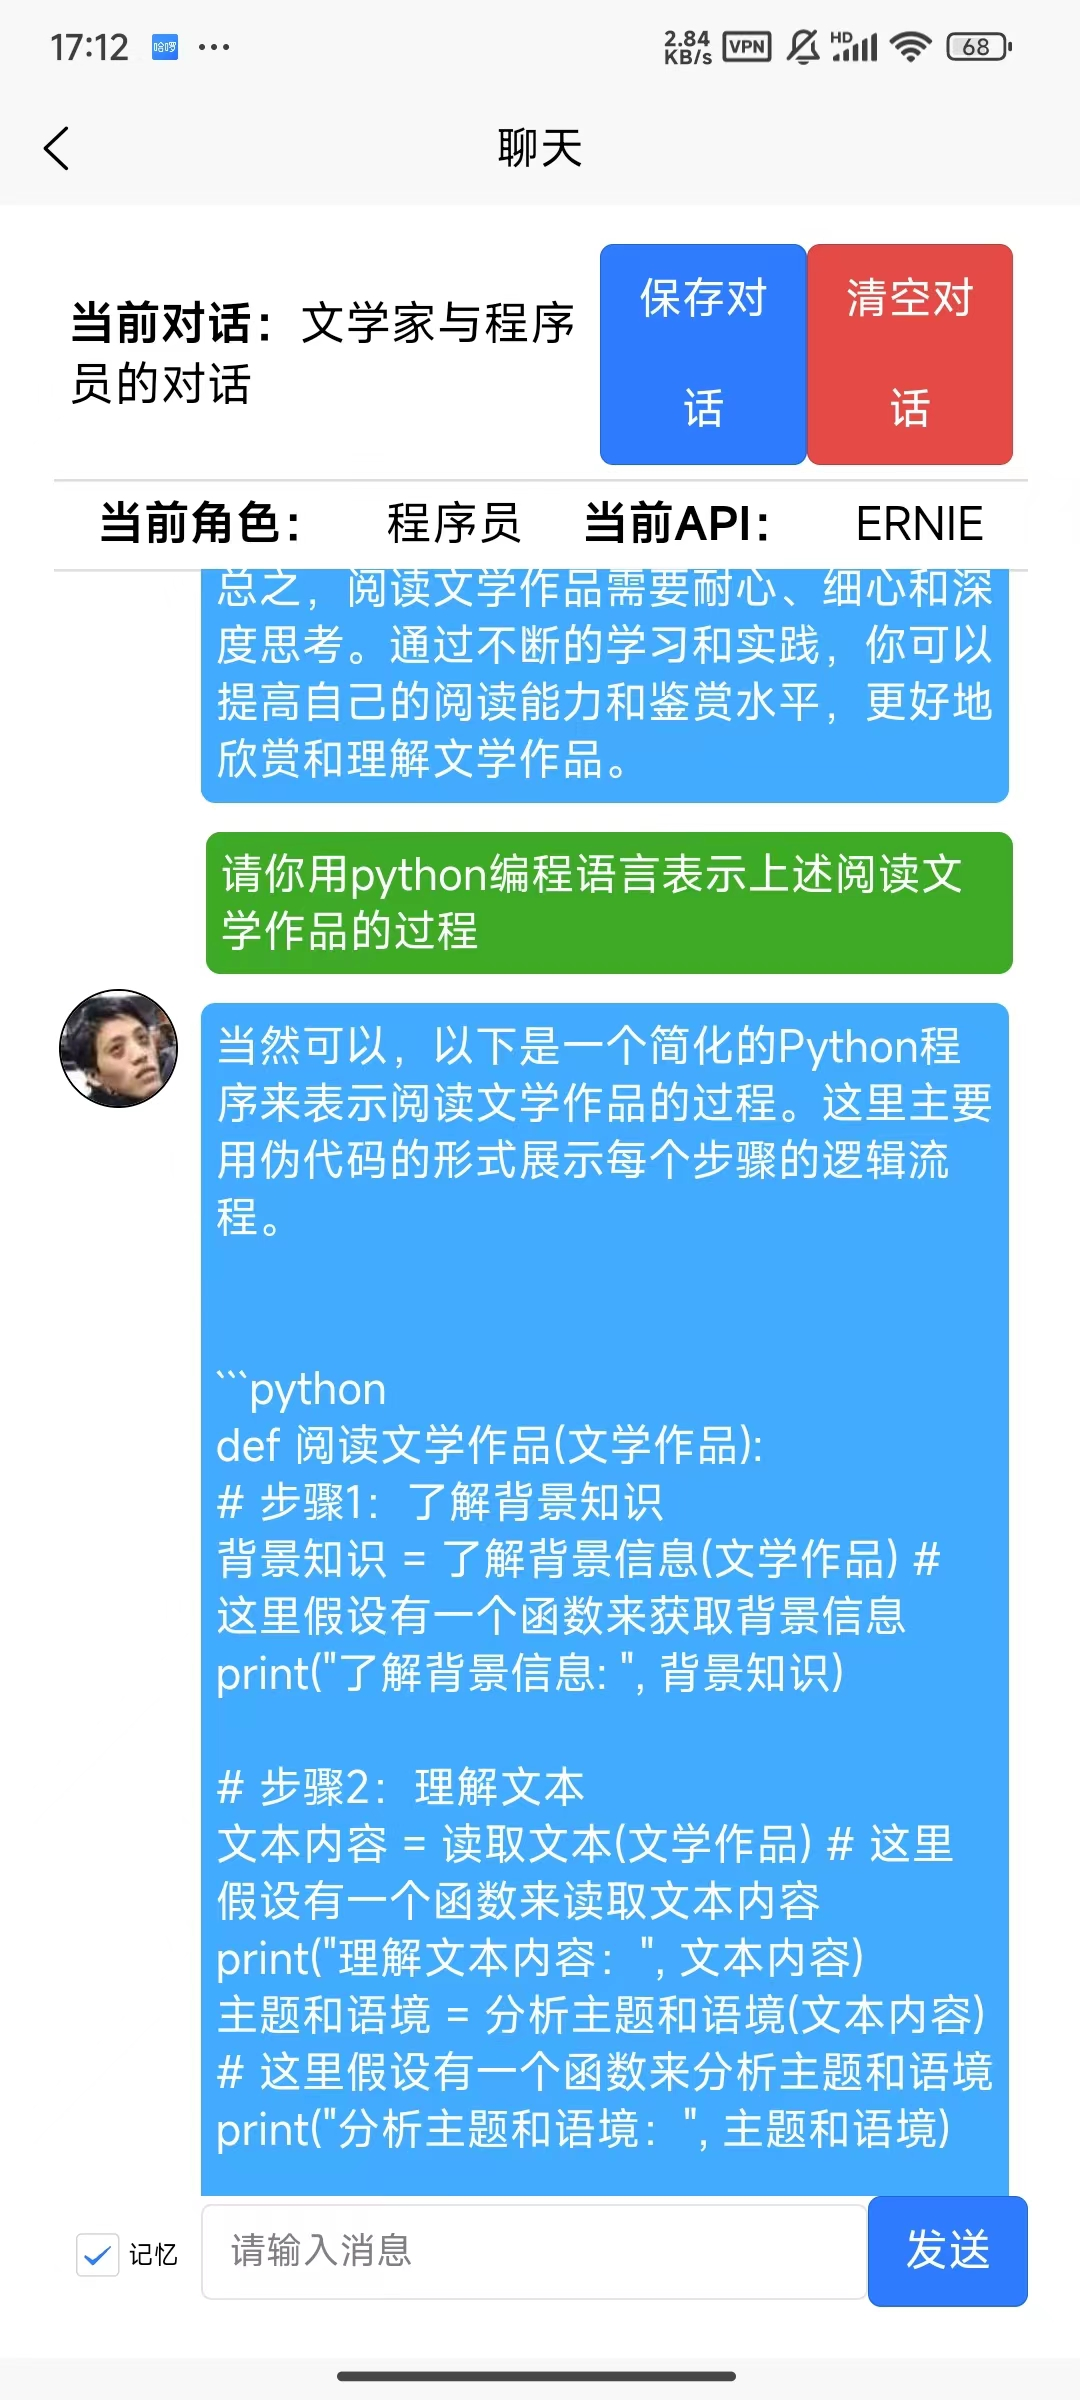
\includegraphics[width=0.4\textwidth]{pics/multi role chat2.jpg}}
    \caption{Chat Free APP多角色聊天}
    \label{fig:multi_role_chat}
\end{figure}

此外,Chat Free APP还支持多角色聊天,用户可以随时切换不同的角色进行聊天,实现多角色的聊天体验。如图\ref{fig:multi_role_chat}所示,用户可以在聊天页面切换不同的角色,发送和接收消息。图中,文学家对阅读文学作品的方式进行了描述,程序员则用代码的形式表示了上述描述的过程。

\newpage
\subsection{记忆功能}

% pics/memory1.jpg, pics/memory2.jpg
\begin{figure}[h]
    \centering
    \subfloat[勾选记忆]{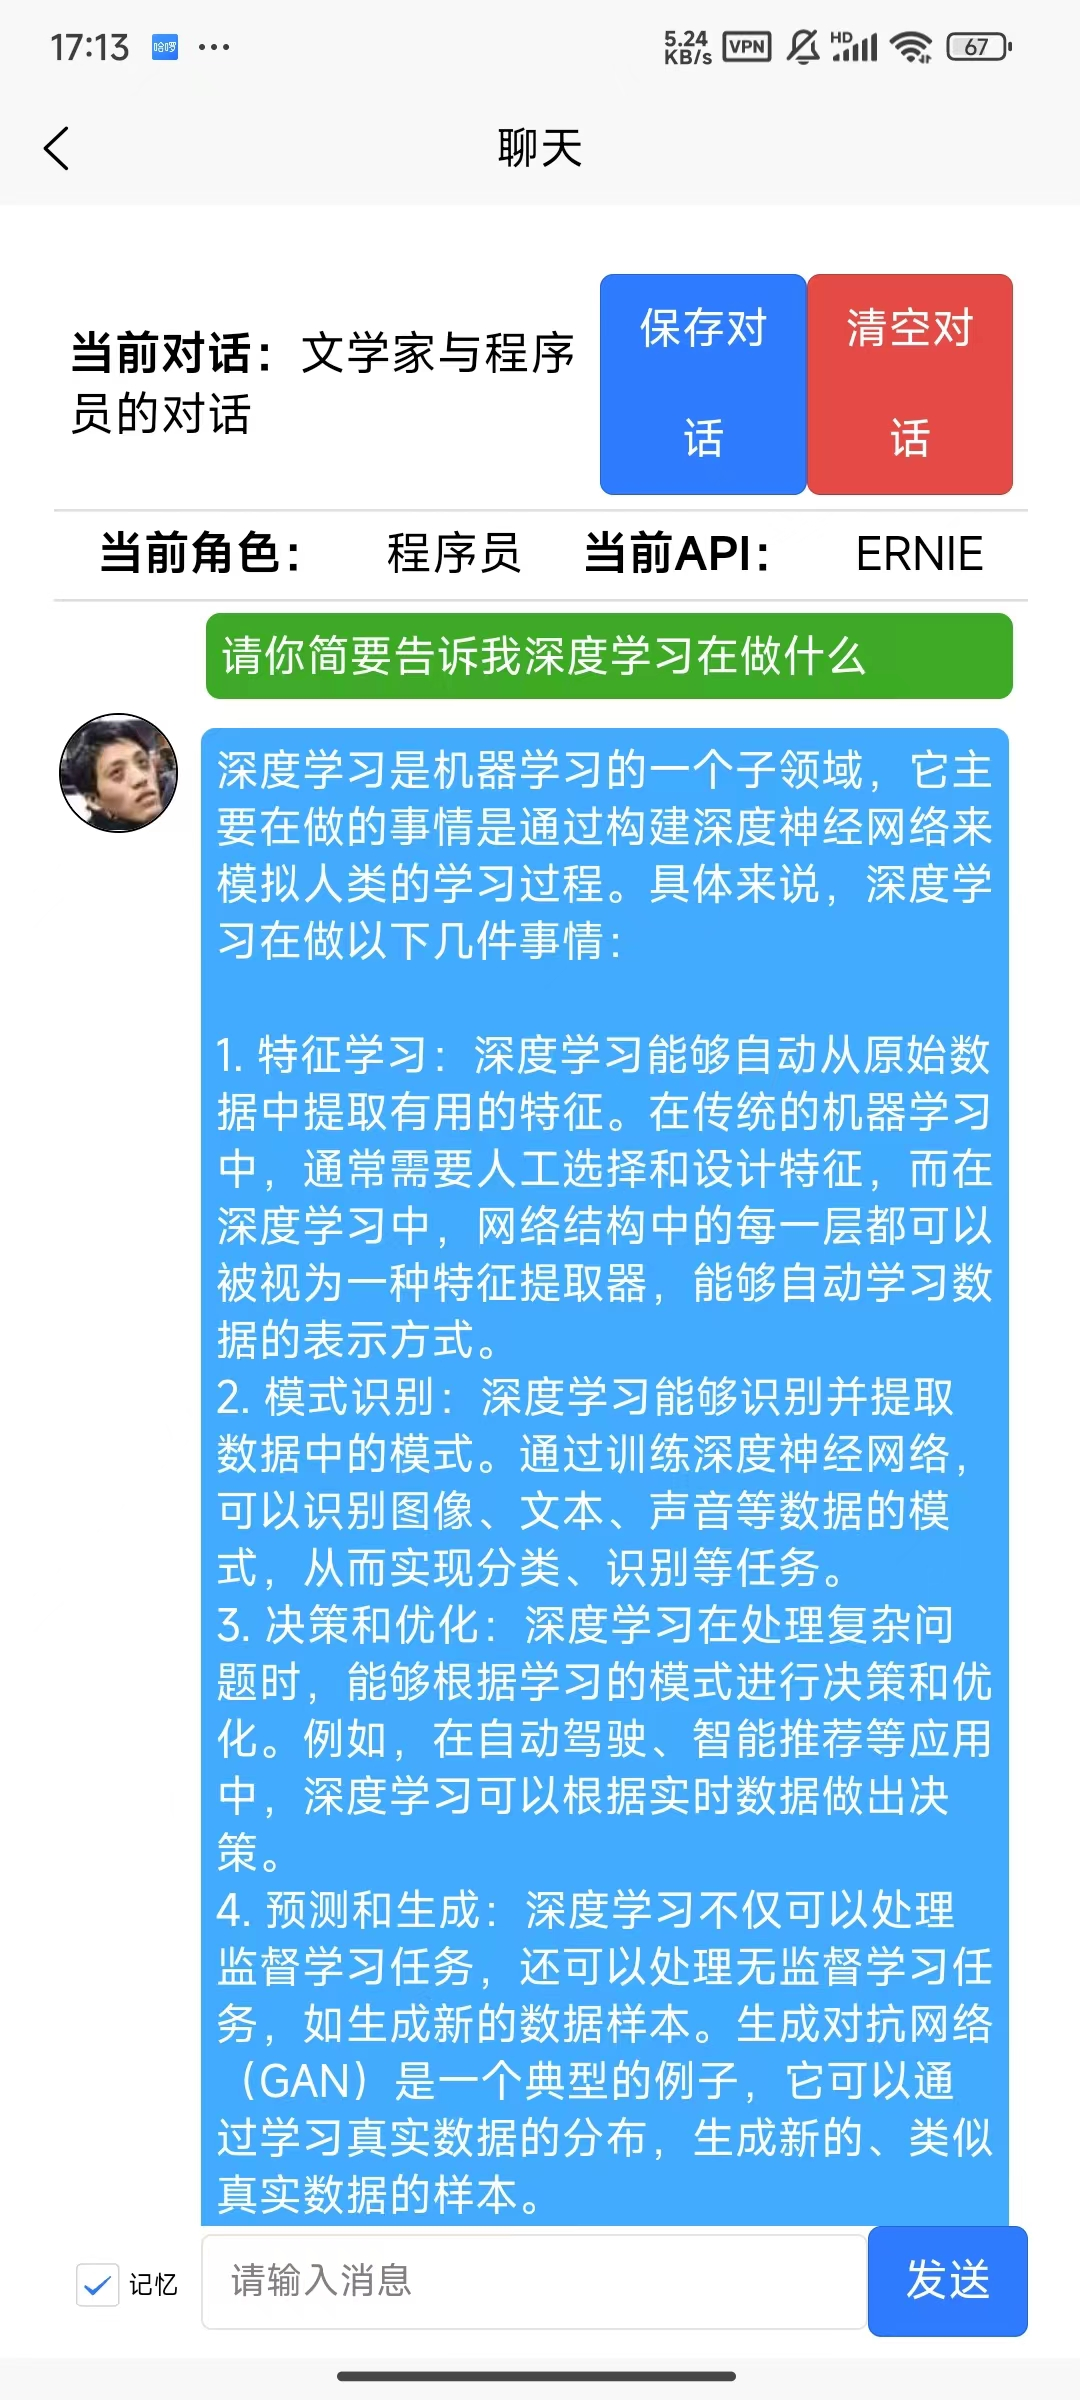
\includegraphics[width=0.38\textwidth]{pics/memory1.jpg}}
    \subfloat[不勾选记忆]{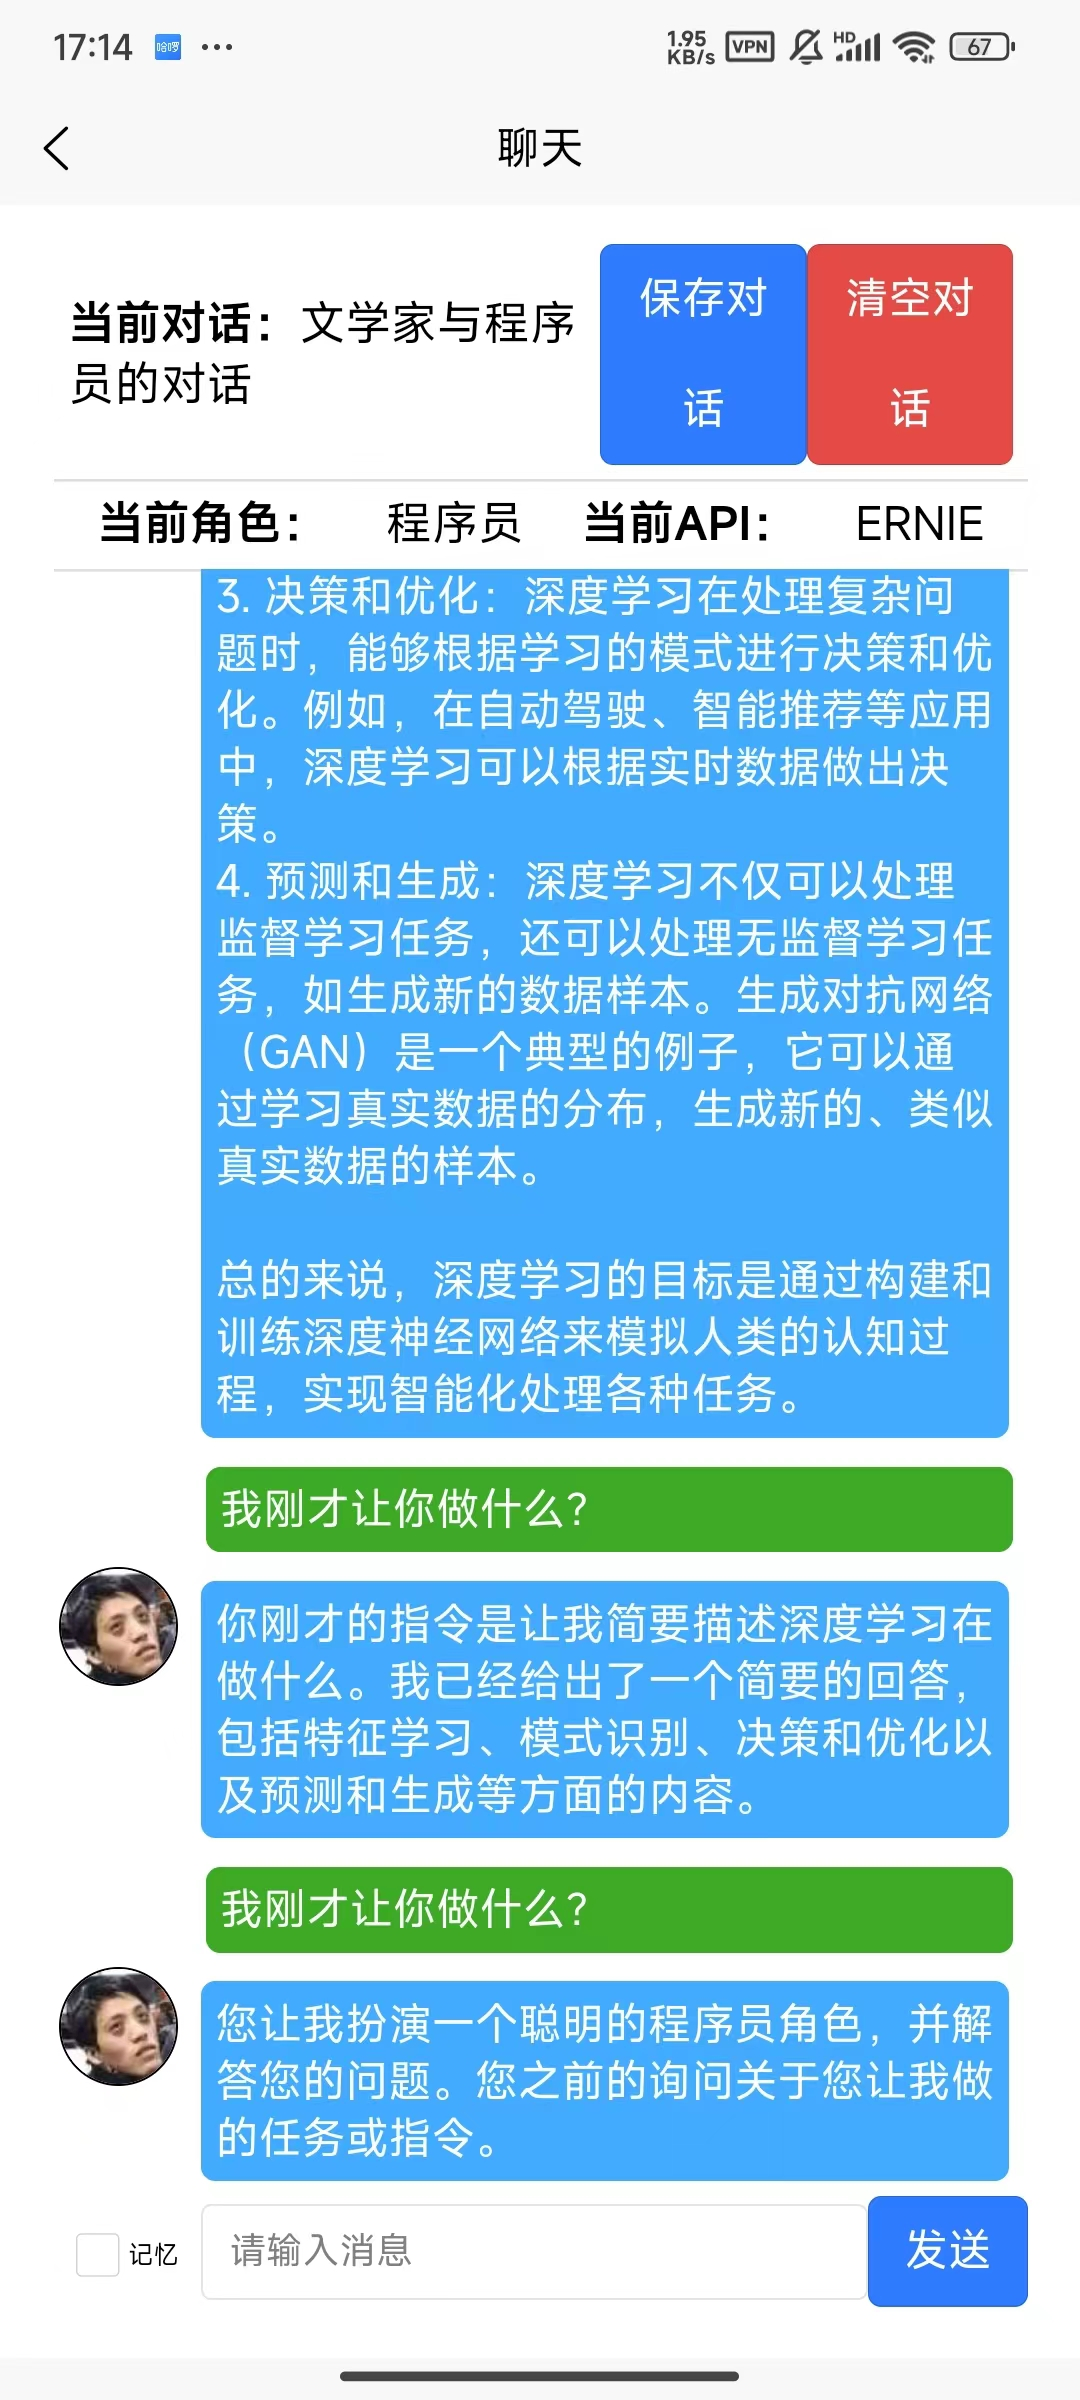
\includegraphics[width=0.38\textwidth]{pics/memory2.jpg}}
    \caption{Chat Free APP记忆功能}
    \label{fig:memory}
\end{figure}

Chat Free APP还支持记忆功能,用户可以选择让LLM是否记忆先前的对话,从而作出不同的反应。如图\ref{fig:memory}所示,当用户勾选记忆时,程序员角色给出的回答是“你刚才的指令是然我简要描述深度学习在做什么”,而当用户不勾选记忆时,程序员角色给出的回答是“您让我扮演一个程序员角色”,忘记了用户的问题。

\section{总结}

Chat Free APP是一款全平台的AI聊天APP,支持不同大语言模型API的调用,用户可以定义不同的角色,实现多角色聊天。本APP具有高度定制化的角色、灵活调节的API、多角色随时切换的聊天、对话历史、记忆功能、多平台支持、免费使用等特点。Chat Free APP基于Vue3、Vite、Uniapp等开发,支持百度ERNIE、讯飞Spark等API。用户可以在APP中定义角色、设置API、创建对话、角色聊天、多角色聊天、记忆功能等。希望Chat Free APP能够给用户带来全新的聊天体验。

\end{document}